\documentclass[12pt,a4paper]{article}
%-----------------------PACKAGES-----------------------%
\usepackage[top=1in,bottom=1in,left=0.5in,right=0.5in]{geometry}
\usepackage{graphicx}
\usepackage{array}
\usepackage{xcolor}
\usepackage{adjustbox}
\usepackage{titlesec}
\usepackage{lettrine}
\usepackage{svg}
\usepackage{caption}
\usepackage{blindtext}
\usepackage{fancyhdr}
\usepackage{hyperref}
\hypersetup{
    colorlinks=true,
    linkcolor=blue,
    filecolor=magenta,      
    urlcolor=cyan,
    pdftitle={Overleaf Example},
    pdfpagemode=FullScreen,
    }


%-----------------------TABLES ALIGNEMNET-----------------------%
\setlength{\tabcolsep}{18pt}
\renewcommand{\arrystretch}{1.5}
\setlength{\arrayrulewidth}{0.5mm}
\setcounter{secnumdepth}{4}

\titleformat{\paragraph}
{\normalfont\normalsize\bfseries}{\theparagraph}{1em}{}
\titlespacing*{\paragraph}
{0pt}{3.25ex plus 1ex minus .2ex}{1.5ex plus .2ex}


%-----------------------TITLE DOCUMENT-----------------------%
% \pagenumbering{roman}
\begin{document}
\begin{Titlepage}
\begin{center}
    \vspace*{2cm}
    \textbf{\Huge  Final Year Project}\\
    \vspace*{1cm}
    \textbf{\Large  UML Class Diagram Compiler}\\
    \vspace*{1cm}
    
      \textbf{ \large FYP Group}
      \vspace{0.2cm}
      \begin{center}
           \large Mehroz Ahmad 18F-0159 \\Wahaj Tahir 19F-1014 \\Ahmad Yasir 19F-0182
      \end{center}
    
    \vspace{1.5cm}
    
    \textbf{\large Supervised \\
    \vspace{0.3cm}\large By}\\
    \vspace{0.2cm}
    \begin{center}
           \large Dr.Sajid Anwer
      \end{center}
       \vspace*{2cm}
      \begin{figure}[hb]
        \centering
        
\includegraphics[scale=0.20]{Fast-Nuces.png}
    \end{figure}
    \vfill
    \vspace{0.8cm}
     Department of Computer Science\\ National University of Computer and Emerging Science\\ Chiniot Faisalabad Campus, Pakistan\\ 2023
    \end{center}

\end{Titlepage}
\pagestyle{empty}

\clearpage
%-----------------------TABLE OF CONTENT-----------------------% 
% \pagenumbering{roman}
\pagestyle{fancy}
\fancyhf{}
\fancyhead[R]{\thepage}
\setcounter{page}{1}
\tableofcontents
\newpage
\listoftables
\newpage
\listoffigures
\clearpage
%-----------------------TABLE OF CONTENT-----------------------% 
\section{Introduction}
UML class diagrams are essential for software development as they provide a visual representation of the structure and relationships among classes in a system. They aid in understanding the system's architecture, facilitating communication among stakeholders, and serving as a blueprint for implementation.
\par In many projects, identifying errors in class diagrams can be a challenging task.There is no definitive method for error detection in class diagrams, and the process can be time-consuming. Additionally, it can be difficult to recall previously made errors, leading to potential repetition of mistakes.
\par To address this challenge, we are embarking on the development of a web application called the "UML-Class Diagram Compiler."This project aims to assist individuals struggling with error identification in class diagrams. The application will take a diagram as input, analyze it based on the established model, and identify the syntactic and semantic errors within the class diagram. Moreover,it will maintain a record of identified errors to enhance the quality of artifacts and prevent their recurrence in the future.
\section{Vision Document}
In this section, the project vision is discussed in detail.
\subsection{Problem Statement}
\begin{table}[h!]
    \centering
    \caption{Problem Statement}
    \begin{tabular}{|l|p{9cm}|}
        \hline
       \textbf{Problem}  &\textbf{Description}  \\ %end of row
       \hline %creating the row line at top
        \textbf{The problem} &
        In many projects, identifying errors in class diagrams can be a challenging task.There is no definitive method for error detection in class diagrams, and the process can be time-consuming. Additionally, it can be difficult to recall previously made errors, leading to potential repetition of mistakes.
        \\% end of row
        \hline
        \textbf{Affects} & 
        The people related to the IT industry i.e. students, internees, teachers, developers etc... \\%end of row
        \hline
        \textbf{The result of which}&
            They can find errors in class diagrams efficiently and they will also have a record of their past errors on the history page.
        \\%end of row
         \hline
        \textbf{Benefits of}&
         UML-Class Diagram compiler is the platform which is providing solution to syntax,semantic errors and also generating skeleton code.
        \\%end of row
        \hline
    \end{tabular}
\end{table}

\subsection{Business Opportunity}
We are living in an era, in which most people are earning from the IT industry. People are doing business by doing IT-related projects and making their side income. Also, developers are having problems, when they want to find errors in the class diagrams but they could not find errors efficiently, as most of the time when there is an error in the class diagram and they start development, it leads to a big problem for the developer as well as investor. So, there is a huge demand for a platform, which resolves all these problems.


\subsection{Objectives}
\begin{itemize}
    \item A system where IT-related people will be able to find errors in class diagrams efficiently without the help of an expert.
    \item A user can also view his/her past errors and improve artifacts in the future.
\end{itemize}

\subsection{Scope}
UML-Class Diagram compiler is a framework for automatic transformation of UML diagram into a string and then compilation of that string for syntactic correctness and verification, which is kind of semantic verification. The compiler will also produce the skeleton code of the given class diagram. The framework is divided into 3 parts.
\begin{enumerate}
    \item \textbf{XML to string converter:} This module will convert the XML form of UML diagram into a string that will follow the context free grammar.
    \item \textbf{UML compiler:} This module will check the syntactic correctness of the diagram and verification of consistency among the diagrams. 
    \item \textbf{Code generator:} This module will allow user to generate the skeleton code of the given class diagram. 
\end{enumerate}
\subsection{Constraints}
	\begin{itemize}
	\item The system shall not require any hardware development or procurement.
    \item The system shall take class diagram as an input in XML format.
    \item The system shall use SQL relational database.
    \item The system shall check the ambiguity and validation of class diagram.
    \item The system shall produce a skeleton code of the UML class diagram.
    \item If there is an internet problem, then might be simple web page will be loaded without graphics.
    \item If the amount of memory available in device is low, the system may ask your application to shut down or sacrifice cached data, slowing program execution.
	\end{itemize}
	
\subsection{Stakeholder and User Descriptions}
	Stakeholder and User Descriptions are defined in detail below.
\subsubsection{Market Demographics}
	Initially, our target market is Pakistan to provide a better platform for developers to find errors in class diagrams efficiently. The IT industry is growing day by day and it has much potential. To overcome this issue, we aim to design a “UML-Class Diagram compiler”, which is a dedicated website for developers.
\newpage	
\subsubsection{Stakeholder Summary}
\begin{table}[h!]
\caption{Stakeholder Summary}
    \centering
    \begin{tabular}{|p{3cm}|p{7cm}|p{5cm}|}
    \hline
       \textbf{Name}  &\textbf{Description} &\textbf{Responsibilities}  \\%end of row
       \hline
         \textbf{Class Diagram Developer}&It includes those who are involved in designing and implementing this project.&
         \newline \textbf{1.} Should design website considering users’ needs.
         \newline \textbf{2.} Proper testing should be applied.
         \newline \textbf{3.} Should be deployed properly.\\%end of row
         \hline
         \textbf{End-users}&End users include all the people related to IT from anywhere in Pakistan.&
         \textbf{1.} Should know using the website\\%end of row
         \hline
         \textbf{Supervisor of project}&Supervisor will be stakeholders of this product as they are involved in the development process of this project with the development team.& 
        \newline\textbf{1.} Gives direction to the development team.
         \newline\textbf{2.} Ensures that the system will be maintainable.
         \newline\textbf{3.} Ensures that there will be market demand for the product’s features.
         \newline\textbf{4.} Monitors the project’s progress.
         \newline\textbf{5.} Ensures that the project complies with the documents generated during project planning and that work products are properly delivered.\\%end of row 
         \hline
    \end{tabular}
\end{table}
\subsubsection{User Environment}
Web-based UML class diagram compiler typically includes the following components:
\begin{enumerate}
    \item\textbf{ Web Browser:}The compiler is accessed through a web browser, which must be compatible with the compiler's interface and features. Popular web browsers used for web-based UML class diagram compilers include Google Chrome, Mozilla Firefox, and Microsoft Edge.
    \item \textbf{Internet Connection:} Since the compiler is web-based, it requires a stable internet connection to access and use the tool.
    \item\textbf{ Operating System:}The operating system used by the developer is not as important for a web-based compiler since the tool is accessed through the browser. However, the browser must be compatible with the developer's operating system.
    \item\textbf{ Hardware:}The computer hardware used by developers should meet the minimum requirements specified by the compiler, such as processor speed, memory, and storage space.
    \item \textbf{Development Environment:}Depending on the web-based compiler, it may need to be integrated with the developer's preferred development environment, such as Eclipse, Visual Studio, or IntelliJ IDEA.
\end{enumerate}

\newpage\subsubsection{Stakeholder Profiles}
The Stakeholder Profiles Attributes of the system are listed in this section.
\paragraph{Supervisors of the Project}%----------------------------------------------------2.6.4.1
\begin{table}[ht]
\caption{Supervisors of the project}
    \centering
    \begin{tabular}{|l|p{7cm}|}
    \hline
       \textbf{Representatives}  &\textbf{Supervisor:}
       Dr.Sajid Anwer
\newline \textbf{Co-supervisor:}  Mr.Asif Ameer   \\%end  of row
       \hline
         \textbf{Description}&They are involved in supervising the activities of the development process. \\%end of row
         \hline
         \textbf{Type}&They are technical stakeholders. They have expertise in domains that are being applied to this project.\\%end of row
         \hline
         \textbf{Responsibilities}&
        \textbf{1.}Gives direction to the development team. 
    \newline\textbf{2.}Ensures that the system will be maintainable. 
    \newline\textbf{3.}Ensures that there will be a market demand for the product’s features. 
    \newline\textbf{4.}Monitor the project’s progress. 
    \newline\textbf{5.}Ensures that the project complies with the documents generated during project planning and that work products are properly delivered. 
    \newline\textbf{6.}They will facilitate the development team to complete this project within specified resources.\\%votes 
    \hline
         \textbf{Success Criteria }&The completion of the feature being committed by the development team at the start of the project. \\%end of row 
         \hline
         \textbf{Involvement}&
         \newline\textbf{1.}Requirement reviewer 
         \newline\textbf{2.}Senior managers 
         \newline\textbf{3.}Reviews implementation  \\%end of row 
         \hline
    \end{tabular}
\end{table}
\vfill
\newpage

\paragraph{Development Team of the Project}
\begin{table}[h!]
\caption{Development Team of the Project}
    \centering
    \begin{tabular}{|l|p{7cm}|}
    \hline
       \textbf{Representative}&\textbf{Mehroz Ahmad}
\newline\textbf{Wahaj Tahir}
\newline\textbf{Ahmad Yasir} \\%end of row
\hline
\textbf{Description}&They are involved in the development process of this project with the
development team. \\%end of row
\hline
\textbf{Type}&They are technical stakeholders.\\%end of row
\hline
\textbf{Responsibilities}&
\newline\textbf{1.} Should design this website considering user’s needs.
\newline\textbf{2.} Proper testing should be applied to make it as effective as possible.\\%end of row
\hline
\textbf{Success Criteria}&The completion of features that are being committed by the development team at the start of the project.\\%end of row
\hline
\textbf{Involvement}&\textbf{1.} Designers
\newline\textbf{2.} Testers\\%end of row
\hline
\textbf{Deliverable}&
\textbf{1.} Documentation
\newline\textbf{2.} Implementation
\newline\textbf{3.} Data acquisition
\newline\textbf{4.} System Training \\%end of row
\hline
    \end{tabular}
\end{table}

\section{System Requirement Specification}
In this section, the features and requirements of the system are explained.
\subsection{System Features}
\begin{enumerate}
    \item Person login
    \item Take XML format input
    \item Convert String
    \item Check the syntactic error
    \item Check the semantic  error
    \item Save error
    \item Generate skeleton code
    
\end{enumerate}

\newpage
\subsection{Functional Requirements}
\begin{table}[h!]
\caption{Functional Requirements}
    \centering
    \begin{tabular}{|l|p{7cm}|}
    \hline
       \textbf{Functionality No.}&\textbf{Description} \\ %end of row
       \hline
       \textbf{FR-1}&
      This application will provide a dedicated page where users can either log in to their existing accounts or sign up for new ones.\\ %end of row
       \hline
       \textbf{FR-2}&
        This application will accept input in the form of XML format files.\\ %end of row
       \hline
       \textbf{FR-3}&
        This application will transform the XML file into a string format.\\ %end of row
       \hline
       \textbf{FR-4}&
        This application will incorporate context-free grammar rules..\\ %end of row
       \hline
       \textbf{FR-5}&
        Using context-free grammar rules, this application will verify and identify syntax and semantic errors in the provided input.\\ %end of row
       \hline
       \textbf{FR-6}&
        This application will automatically generate a skeleton code structure of provided input.\\ %end of row
       \hline
       \textbf{FR-7}&
        This application will include a history page that will maintain a record of the user's previous mistakes for reference and review.\\ %end of row
       \hline
       \textbf{FR-8}&
       The administrator will have the ability to add words in natural language to the system.\\ %end of row
       \hline
       \textbf{FR-9}&
        The administrator will have the capability to define the natural language using context-free grammar in the system.\\ %end of row
       \hline
       \textbf{FR-10}&
       The administrator will have the authority to implement and configure the rules in the system.\\ %end of row
       \hline   
    \end{tabular}
\end{table}

\newpage
\subsection{Non-Functional Requirements}
\begin{table}[h!]
\caption{Non-Functional Requirements}
    \centering
    \begin{tabular}{|l|p{7cm}|}
    \hline
       \textbf{Non-Functionality}&\textbf{Description} \\ %end of row
       \hline
       \textbf{NFR-1}&
The application should be active to response 24 hours a day and 7 days a week.\\ %end of row
       \hline
       \textbf{NFR-2}&
       The UML class diagram compiler should provide a user-friendly interface with clear instructions and intuitive navigation.
\newline• The application should have a user satisfaction rating of at least 60\% based on user surveys or feedback.
\newline• The average time for users to learn and become proficient in using the compiler should be less than 1 hour.\\ %end of row
       \hline
       \textbf{NFR-3}&
       The average time to fix bugs or address issues reported by users should be less than 3 days.\\ %end of row
       \hline
       \textbf{NFR-4}&
        The UML class diagram compiler should have a low error rate, ensuring that it correctly identifies syntax and semantic errors in class diagrams at least 75\% of the time.\\ %end of row
       \hline
       \textbf{NFR-5}&
        The UML class diagram compiler should be able to handle an increasing number of class diagrams and users without significant degradation in performance. It should support a concurrent user load of at least 5 users.\\ %end of row
       \hline
       \textbf{NFR-6}&
       The application should have a response time of less than 1.5 milliseconds for user interactions such as login, sign-up, or diagram validation.\\ %end of row
       \hline
       \textbf{NFR-7}&
       The application should undergo regular security assessments and vulnerability testing to ensure the integrity of the system.\\ %end of row
       \hline
    \end{tabular} 
    \end{table}
    % -------------USE CASE DIAGRAM--------------------------------------------------------------
    \clearpage
    \section{Use Case Diagram}

    \begin{figure}[h]
        \centering
      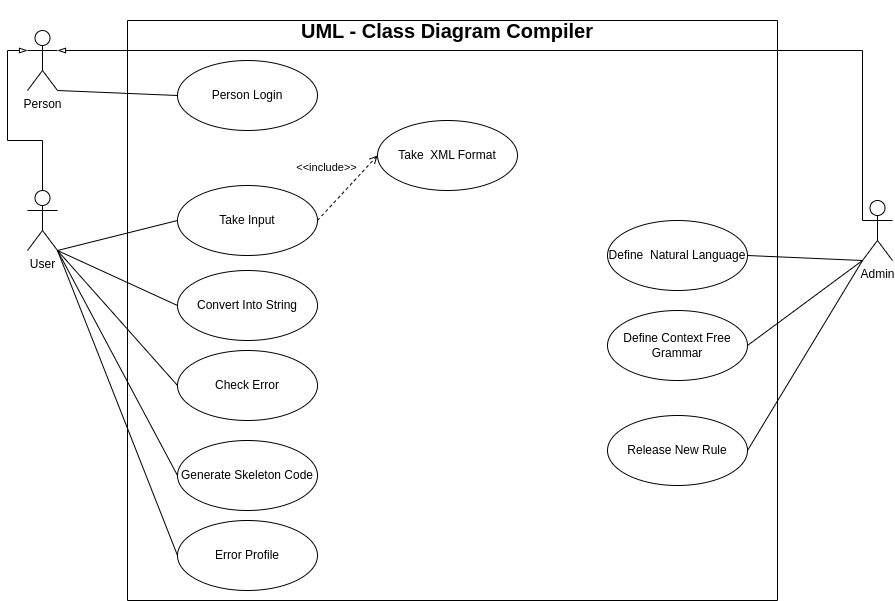
\includegraphics[width=\textwidth]{Diagram/use case diagram.png}
      \caption{Use case Diagram}
    \end{figure}

    % -------------HIGH LEVEL USE-CASES--------------------------------------------------------------
% \section{High-level use cases}
% \subsection{Person Login}
% \begin{table}[h!]
% \caption{Person Login}
%     \centering
%     \begin{tabular}{|l|p{7cm}|}
%     \hline
%        \textbf{Use case ID}&01 \\ %end of row
%        \hline
%        \textbf{Use case Name}&Person Login \\ %end of row
%        \hline
%        \textbf{Actor}&User \\ %end of row
%        \hline
%        \textbf{Description}&To use the application, the user must create an account. If he already has the account, he will log in, and to manage the application, the admin needs an account by signing up, and if he already has one, sign in. \\ %end of row
%        \hline
%     \end{tabular} 
%     \end{table}

% \subsection{Take Input}
% \begin{table}[h!]
% \caption{Take Input}
%     \centering
%     \begin{tabular}{|l|p{7cm}|}
%     \hline
%        \textbf{Use case ID}&02 \\ %end of row
%        \hline
%        \textbf{Use case Name}&Take Input \\ %end of row
%        \hline
%        \textbf{Actor}&User \\ %end of row
%        \hline
%        \textbf{Description}&The user would have to give input to the system in an XML format which will proceed the system further.\\ %end of row
%        \hline
%     \end{tabular} 
%     \end{table}
    
% \subsection{Take XML Format}
% \begin{table}[h!]
% \caption{Take XML Format}
%     \centering
%     \begin{tabular}{|l|p{7cm}|}
%     \hline
%        \textbf{Use case ID}&03 \\ %end of row
%        \hline
%        \textbf{Use case Name}&Take XML Format \\ %end of row
%        \hline
%        \textbf{Actor}&User \\ %end of row
%        \hline
%        \textbf{Description}&The system will take the XML format, convert it into a string, and perform error-checking functionalities.\\ %end of row
%        \hline
%     \end{tabular} 
%     \end{table}

% \subsection{Check Syntactic Error}
% \begin{table}[h!]
% \caption{Check Syntactic Error}
%     \centering
%     \begin{tabular}{|l|p{7cm}|}
%     \hline
%        \textbf{Use case ID}&04 \\ %end of row
%        \hline
%        \textbf{Use case Name}&Check syntactic error \\ %end of row
%        \hline
%        \textbf{Actor}&User \\ %end of row
%        \hline
%        \textbf{Description}&The system would find all possible syntactic errors and display those errors on screen.\\ %end of row
%        \hline
%     \end{tabular} 
%     \end{table}
% \clearpage
% \subsection{Convert String}
%     \begin{table}[h!]
% \caption{Convert String}
%     \centering
%     \begin{tabular}{|l|p{7cm}|}
%     \hline
%        \textbf{Use case ID}&05 \\ %end of row
%        \hline
%        \textbf{Use case Name}&Convert String \\ %end of row
%        \hline
%        \textbf{Actor}&User \\ %end of row
%        \hline
%        \textbf{Description}&After giving the input the system will convert the file into a string and make it readable.\\ %end of row
%        \hline
%     \end{tabular} 
%     \end{table}

%     \subsection{Check Semantic Error}
%     \begin{table}[h!]
% \caption{Check Semantic Error}
%     \centering
%     \begin{tabular}{|l|p{7cm}|}
%     \hline
%        \textbf{Use case ID}&06 \\ %end of row
%        \hline
%        \textbf{Use case Name}&Check semantic error \\ %end of row
%        \hline
%        \textbf{Actor}&User \\ %end of row
%        \hline
%        \textbf{Description}&The system will check the semantic errors if there are any and make information about those mistakes.\\ %end of row
%        \hline
%     \end{tabular} 
%     \end{table}
    
%     \subsection{Generate Skeleton Code}
%     \begin{table}[h!]
% \caption{Generate Skeleton Code}
%     \centering
%     \begin{tabular}{|l|p{7cm}|}
%     \hline
%        \textbf{Use case ID}&07 \\ %end of row
%        \hline
%        \textbf{Use case Name}&Generate Skeleton Code \\ %end of row
%        \hline
%        \textbf{Actor}&User \\ %end of row
%        \hline
%        \textbf{Description}&After converting the input into the string, the user can generate its skeleton code by just clicking on generate skeleton code.\\ %end of row
%        \hline
%     \end{tabular} 
%     \end{table}
%     \clearpage

%      \subsection{Error Profile}
%     \begin{table}[h!]
% \caption{Error Profile}
%     \centering
%     \begin{tabular}{|l|p{7cm}|}
%     \hline
%        \textbf{Use case ID}&08 \\ %end of row
%        \hline
%        \textbf{Use case Name}&Error Profile \\ %end of row
%        \hline
%        \textbf{Actor}&User \\ %end of row
%        \hline
%        \textbf{Description}&The user’s work will save on the history page and the user can review his/her errors. It is used for just keeping track of users’ past mistakes.\\ %end of row
%        \hline
%     \end{tabular} 
%     \end{table}
    
% \subsection{Define Natural Language}
% \begin{table}[h!]
% \caption{Define Natural Language}
%     \centering
%     \begin{tabular}{|l|p{7cm}|}
%     \hline
%        \textbf{Use case ID}&09 \\ %end of row
%        \hline
%        \textbf{Use case Name}&Define Natural Language \\ %end of row
%        \hline
%        \textbf{Actor}&Admin \\ %end of row
%        \hline
%        \textbf{Description}&When an admin wants to add some new sentences to the system. He will click on the add sentence button and type the sentence he/she wants.\\ %end of row
%        \hline
%     \end{tabular} 
%     \end{table}
%      \subsection{Define CFG’s}
%     \begin{table}[h!]
% \caption{Define CFG’s}
%     \centering
%     \begin{tabular}{|l|p{7cm}|}
%     \hline
%        \textbf{Use case ID}&10 \\ %end of row
%        \hline
%        \textbf{Use case Name}&Define CFG’s \\ %end of row
%        \hline
%        \textbf{Actor}&Admin \\ %end of row
%        \hline
%        \textbf{Description}&The admin who right the sentence must it according to the CFG rules, to make it understandable by the system by clicking on the define in CFG rule button will make the sentence according to the CFG rules.\\ %end of row
%        \hline
%     \end{tabular} 
%     \end{table}

% \clearpage
%       \subsection{Implement the Rule}
%     \begin{table}[h!]
% \caption{Implement the Rule}
%     \centering
%     \begin{tabular}{|l|p{7cm}|}
%     \hline
%        \textbf{Use case ID}&11 \\ %end of row
%        \hline
%        \textbf{Use case Name}&Implement Rule \\ %end of row
%        \hline
%        \textbf{Actor}&Admin \\ %end of row
%        \hline
%        \textbf{Description}&The sentence which is arranged and correct according to the CFG rule will now be implemented in the system.\\ %end of row
%        \hline
%     \end{tabular} 
%     \end{table}
 % -------------EXPENDED USE CASES------------------------------------------------------------------
\newpage
\section{Expended use cases}
\subsection{Person Login}
\begin{table}[h!]
\caption{ECU-01 Person Login}
    \centering
    \begin{tabular}{|l|p{10cm}|}
    \hline
       \textbf{Use case ID}&01 \\ %end of row
       \hline
       \textbf{Use case Name}&Person Login\\ %end of row
       \hline
       \textbf{Actor}&Person \\ %end of row
       \hline
       \textbf{Description}&To use the application, the user must create an account. If he already has the account, he will log in, and to manage the application, the admin needs an account by signing up, and if he already has one, sign in. \\ %end of row
       \hline
       \textbf{Trigger}&The user has requested to login. \\ %end of row
        \hline
       \textbf{Pre-Condition}&
   \newline • User/Admin has an active internet connection.
   \newline • User/Admin has a web browser
   \newline • User/Admin will go to the website
   \newline • User/Admin will type the credentials
\\ %end of row
        \hline
       \textbf{Post-Condition}&• Login successfully \\ %end of row
        \hline
       \textbf{Normal Flow}&
    \textbf{1.}Users/Admins access the UML class diagram compiler web application through a web browser or dedicated client interface.
\newline  \textbf{2.}Existing users navigate to the login page.Users/Admins enter their registered username/email and password in the provided fields.
\newline \textbf{3.}New users navigate to the signup page.Users enter their desired username, email, and password in the respective fields.
 \newline \textbf{4.}After login or signup, the system redirects the user to their dashboard or main page.\\ %end of row
\hline
       \textbf{Alternate Flow}&
       \textbf{2.1.}If the user enters incorrect login credentials, such as an invalid username or password, the system displays an error message indicating an unsuccessful login attempt.
\newline\textbf{3.1.}During the signup process, the system may check for duplicate accounts with the same email or username.
\newline\textbf{4.1.}After resolving these issues the system redirects the user to their dashboard or main page.\\ %end of row
        \hline
       \textbf{Special Requirement}&Availability of Internet \\ %end of row
        \hline
       \textbf{Frequency of Use}&High \\ %end of row
        \hline
       \textbf{Assumption}&The user knows how to log in. \\ %end of row
       \hline
    \end{tabular} 
    \end{table}


\clearpage
 \subsection{Take Input}
\begin{table}[h!]
\caption{ECU-02 Take Input}
    \centering
    \begin{tabular}{|l|p{10cm}|}
    \hline
       \textbf{Use case ID}&02 \\ %end of row
       \hline
       \textbf{Use case Name}&Take Input \\ %end of row
       \hline
       \textbf{Actor}&User \\ %end of row
       \hline
       \textbf{Description}&The user would have to give input to the system in an XML format which will proceed the system further.\\ %end of row
       \hline
       \textbf{Trigger}&The user has clicked to give the upload file. \\ %end of row
        \hline
       \textbf{Pre-Condition}&
   \newline• The user has logged in successfully.
    \newline• User must be in the application
\\ %end of row
        \hline
       \textbf{Post-Condition}&• The given file will be uploaded for evaluation.
 \\ %end of row
        \hline
       \textbf{Normal Flow}&
    \textbf{1.}The user creates or obtains a valid XML file containing the UML class diagram representation.
\newline\textbf{2.}Within the application, there is an option to select or upload the input file.
\newline\textbf{3.}The UML class diagram compiler parses and reads the content of the input file.\\ %end of row
\hline
       \textbf{Alternate Flow}&
       \textbf{1.1.}If the user attempts to upload a file that does not adhere to the required format.It will throw an error.
\newline\textbf{2.1.}The user is informed about the missing or incomplete data and may be prompted to provide the necessary information or correct the existing data.
\newline\textbf{3.1.}In the case of encountering unrecognized elements or unsupported UML constructs within the input file, the compiler raises warnings.\\ %end of row
        \hline
       \textbf{Special Requirement}&Availability of file in XML format \\ %end of row
        \hline
       \textbf{Frequency of Use}&High \\ %end of row
        \hline
       \textbf{Assumption}&The user knows how to upload a file \\ %end of row
       \hline
    \end{tabular} 
    \end{table}


\clearpage
    \subsection{Take XML Format}
\begin{table}[h!]
\caption{ECU-03 Take XML Format}
    \centering
    \begin{tabular}{|l|p{10cm}|}
    \hline
       \textbf{Use case ID}&03 \\ %end of row
       \hline
       \textbf{Use case Name}&Take XML Format \\ %end of row
       \hline
       \textbf{Actor}&User \\ %end of row
       \hline
       \textbf{Description}&The system will take the XML format, convert it into a string, and perform error-checking functionalities.\\ %end of row
       \hline
       \textbf{Trigger}&Giving input to the system\\ %end of row
        \hline
       \textbf{Pre-Condition}&
   \newline • User must be in the system
    \newline • The file must be in XML format
\\ %end of row
        \hline
       \textbf{Post-Condition}& • File is uploaded successfully
 \\ %end of row
        \hline
       \textbf{Normal Flow}&
    \textbf{1.}The user creates or obtains a valid XML file containing the UML class diagram representation.
\newline\textbf{2.}Within the application, there is an option to select or upload the input file.
\newline\textbf{3.}The UML class diagram compiler parses and reads the content of the input file. \\ %end of row
\hline
       \textbf{Alternate Flow}&
        \textbf{1.1.}If the user attempts to upload a file that does not adhere to the required format.It will throw an error.
\newline\textbf{2.1.}The user is informed about the missing or incomplete data and may be prompted to provide the necessary information or correct the existing data.
\newline\textbf{3.1.}In the case of encountering unrecognized elements or unsupported UML constructs within the input file, the compiler raises warnings.\\ %end of rows %end of row
        \hline
       \textbf{Special Requirement}&The user should click on the input icon \\ %end of row
        \hline
       \textbf{Frequency of Use}&High \\ %end of row
        \hline
       \textbf{Assumption}&The user should know how to give input in XML format. \\ %end of row
       \hline
    \end{tabular} 
    \end{table}


\newpage  
    \subsection{Convert Into String}
    \begin{table}[h]
\caption{ECU-04 Convert Into String}
    \centering
    \begin{tabular}{|l|p{10cm}|}
    \hline
       \textbf{Use case ID}&05 \\ %end of row
       \hline
       \textbf{Use case Name}&Convert String \\ %end of row
       \hline
       \textbf{Actor}&User \\ %end of row
       \hline
       \textbf{Description}&After giving the input the system will convert the file into a string and make it readable.\\ %end of row
       \hline

    \textbf{Trigger}&The user will give input to the system. \\ %end of row
        \hline
       \textbf{Pre-Condition}&
• The user must be in the system
\newline• The file format should be XML
\\ %end of row
        \hline
       \textbf{Post-Condition}&• Convert into string successfully
 \\ %end of row
        \hline
       \textbf{Normal Flow}&\textbf{1.}The user provides an XML file containing the UML class diagram.

\textbf{2.}The UML class diagram compiler parses the XML file, extracting the necessary class diagram information.

\textbf{3.}The string representation may include the class definitions, relationships, attributes, and methods in a readable format. \\ %end of row
\hline
       \textbf{Alternate Flow}&
       \textbf{1.1.}An error message is displayed, indicating the invalid XML format, and the user is prompted to provide a valid XML file in order to make it readable.
\newline\textbf{2.1.}The compiler raises warnings or errors, indicating the missing or incomplete data, and the user is informed about the specific elements that need to be provided or corrected.
\newline\textbf{3.1.}If there are issues during the conversion process, such as unexpected data or errors in the parsed XML, the compiler may encounter difficulties in converting the XML to a string representation.\\ %end of row
        \hline
       \textbf{Special Requirement}&Specific format input \\ %end of row
        \hline
       \textbf{Frequency of Use}&High \\ %end of row
        \hline
       \textbf{Assumption}&The user should know how to upload a file.\\ %end of row
       \hline
    \end{tabular} 
    \end{table}


\clearpage
\subsection{Check Error}
\begin{table}[h!]
\caption{ECU-05 Check Error}
    \centering
    \begin{tabular}{|l|p{10cm}|}
    \hline
       \textbf{Use case ID}&04 \\ %end of row
       \hline
       \textbf{Use case Name}&Check error \\ %end of row
       \hline
       \textbf{Actor}&User \\ %end of row
       \hline
       \textbf{Description}&The system would find all possible syntactic errors and display those errors on screen.\\ %end of row
       \hline
       \textbf{Trigger}&The user has clicked the icon to check the syntactic error \\ %end of row
        \hline
       \textbf{Pre-Condition}&
•  File must be uploaded successfully
\\ %end of row
        \hline
       \textbf{Post-Condition}&• The system will check and display all possible syntactic and semantic errors in the class diagram.
 \\ %end of row
        \hline
       \textbf{Normal Flow}&\textbf{1.}It checks if the elements are properly defined, the relationships are correctly specified, and the syntax rules of UML class diagrams are followed then it follows the instruction semantic rules.
\newline\textbf{2.}During the syntax or semantic error analysis, if any syntax or semantic errors are found, such as missing or misplaced brackets, incorrect notation usage, or invalid element declarations, the compiler identifies them.
\newline\textbf{3.}The UML class diagram compiler presents the syntax and semantic error messages or notifications to the user. \\ %end of row
\hline
\textbf{Alternate Flow}&\textbf{1.1.}The compiler raises warnings or errors, indicating the presence of unsupported notations or constructs, and advises the user to remove or replace them with valid UML syntax.
\newline\textbf{2.2.}If the class diagram has incomplete or partially defined syntax, such as missing element declarations or unfinished relationships, the compiler recognizes the incomplete sections and semantic error can not be resolved.\\ %end of row
        \hline
       \textbf{Special Requirement}&Availability of input \\ %end of row
        \hline
       \textbf{Frequency of Use}&High \\ %end of row
        \hline
       \textbf{Assumption}&The user knows the errors in the class diagram already\\ %end of row
       \hline
    \end{tabular} 
    \end{table}



  

% \clearpage
%     \subsection{Check Semantic Error}
%     \begin{table}[h!]
% \caption{ECU-06 Check Semantic Error}
%     \centering
%     \begin{tabular}{|l|p{10cm}|}
%     \hline
%        \textbf{Use case ID}&06 \\ %end of row
%        \hline
%        \textbf{Use case Name}&Check semantic error \\ %end of row
%        \hline
%        \textbf{Actor}&User \\ %end of row
%        \hline
%        \textbf{Description}&The system will check the semantic errors if there are any and make information about those mistakes.\\ %end of row
%        \hline
%        \textbf{Trigger}&The user will give input to the system. \\ %end of row
%         \hline
%        \textbf{Pre-Condition}&
% \textbf • The user will give input to the system.
% \newline\textbf • File is uploaded and converted to string successfully
% \newline\textbf • The system has checked the syntactic errors
% \\ %end of row
%         \hline
%        \textbf{Post-Condition}&• Display the semantic errors
%  \\ %end of row
%         \hline
%        \textbf{Normal Flow}&
%     \textbf{1.}\textbf{User Input:}The user provides a UML class diagram in XML format.
% \newline \textbf{2.}\textbf{Semantic Analysis:}The UML class diagram compiler performs a semantic analysis on the provided class diagram.
% \newline \textbf{3.}\textbf{Semantic Error Detection:}The compiler generates error messages or notifications indicating the specific semantic errors and their locations within the class diagram.\\ %end of row
% \hline
%        \textbf{Alternate Flow}&\textbf{1.1.}\textbf{Unsupported format:} The compiler raises warnings or errors, indicating the wrong format.\\ %end of row
%         \hline
%        \textbf{Special Requirement}&The syntactic errors should be checked \\ %end of row
%         \hline
%        \textbf{Frequency of Use}&High \\ %end of row
%         \hline
%        \textbf{Assumption}&The user should know how to upload a file.\\ %end of row
%        \hline
%     \end{tabular} 
%     \end{table}


    
  \clearpage  
    \subsection{Generate Skeleton Code}
    \begin{table}[h!]
\caption{ECU-06 Generate Skeleton Code}
    \centering
    \begin{tabular}{|l|p{10cm}|}
    \hline
       \textbf{Use case ID}&07 \\ %end of row
       \hline
       \textbf{Use case Name}&Generate Skeleton Code \\ %end of row
       \hline
       \textbf{Actor}&User \\ %end of row
       \hline
       \textbf{Description}&After converting the input into the string, the user can generate its skeleton code by just clicking on generate skeleton code.\\ %end of row
        \hline
       \textbf{Trigger}&The user will click on generate skeleton code \\ %end of row
        \hline
       \textbf{Pre-Condition}&
\textbf• The file is uploaded in XML format successfully
\newline\textbf• File is converted into string\\ %end of row
        \hline
       \textbf{Post-Condition}&\textbf• Skeleton code is generated
 \\ %end of row
        \hline
       \textbf{Normal Flow}&
    \textbf{1.}Based on the information gathered, the compiler generates skeleton code that represents the structure and basic functionality of the classes in the diagram.

\newline\textbf{2.}The skeleton code may include class definitions, method signatures, variable declarations, and other basic code structures.
\\ %end of row
\hline
       \textbf{Alternate Flow}&
       \textbf{1.1.}In some cases, the class diagram may have ambiguous or conflicting elements that can lead to ambiguous or conflicting code generation.
\newline\textbf{2.2.}The compiler generates an error message indicating the code generation failure and provides guidance to the user for troubleshooting or resolving the issue.\\ %end of row
        \hline
       \textbf{Special Requirement}&User should give some input to check errors. \\ %end of row
        \hline
       \textbf{Frequency of Use}&High \\ %end of row
        \hline
       \textbf{Assumption}&Admin should know basic rules of the class diagram\\ %end of row
       \hline
    \end{tabular} 
    \end{table}


\clearpage
     \subsection{Error Profile}
    \begin{table}[h!]
\caption{ECU-07 Error Profile}
    \centering
    \begin{tabular}{|l|p{10cm}|}
    \hline
       \textbf{Use case ID}&08 \\ %end of row
       \hline
       \textbf{Use case Name}&Error Profile \\ %end of row
       \hline
       \textbf{Actor}&User \\ %end of row
       \hline
       \textbf{Description}&The user’s work will save on the history page and the user can review his/her errors. It is used for just keeping track of users’ past mistakes.\\ %end of row
        \hline
       \textbf{Trigger}&Click on save error button  \\ %end of row
        \hline
       \textbf{Pre-Condition}&
• The user will find errors in the class diagram.
\\ %end of row
        \hline
       \textbf{Post-Condition}&• The errors of class diagram will be saved in his/her profile.
       \newline• The user can also view his/her errors in the class diagram.
 \\ %end of row
        \hline
       \textbf{Normal Flow}&
    \textbf{1.}The user interacts with the UML class diagram compiler, performing various actions such as uploading class diagrams, analyzing code, generating output, etc.
\newline\textbf{2.}The UML class diagram compiler records the user's activities, capturing relevant information such as the actions performed, timestamps, user identification, and any relevant data associated with the activities.
\newline\textbf{3.}The compiler stores the activity logs in a database which can be review later by users.\\ %end of row
\hline
       \textbf{Alternate Flow}&
       \textbf{1.}The compiler may raise warnings or errors, notifying the user about the missing or incomplete logs and suggesting possible actions to rectify the situation.
       \newline\textbf{2.1.}The compiler generates error messages or notifications, informing the user about the logging failures and advising them to retry the action or report the issue to the system administrator.\\ %end of row
        \hline
       \textbf{Special Requirement}&There should be some error found in the class diagram. \\ %end of row
        \hline
       \textbf{Frequency of Use}&High \\ %end of row
        \hline
       \textbf{Assumption}&The user should know how to find errors and save errors. \\ %end of row
       \hline
    \end{tabular} 
    \end{table}

\clearpage
\subsection{Define Natural Language}
\begin{table}[h!]
\caption{ECU-08 Define Natural Language}
    \centering
    \begin{tabular}{|l|p{10cm}|}
    \hline
       \textbf{Use case ID}&09 \\ %end of row
       \hline
       \textbf{Use case Name}&Define Natural Language \\ %end of row
       \hline
       \textbf{Actor}&Admin \\ %end of row
       \hline
       \textbf{Description}&When an admin wants to add some new sentences to the system. He will click on the add sentence button and type the sentence he/she wants.\\ %end of row
        \hline
       \textbf{Trigger}&Click on add sentence button\\ %end of row
        \hline
       \textbf{Pre-Condition}&
 • Admin must be connected to the internet.
\newline• Admin must be logged into the system.
\\ %end of row
        \hline
       \textbf{Post-Condition}&• Arrange sentence according to the CFG rule.
 \\ %end of row
        \hline
       \textbf{Normal Flow}&
    \textbf{1.}The admin type a set of natural language words or phrases that they want to associate with specific elements or concepts in the UML class diagram compiler.

\newline\textbf{2.}The admin will type the set of words or sentence and then add them.\\ %end of row
\hline
       \textbf{Alternate Flow}&
       \textbf{1.1.}Sentences starting with numbers or special characters generate an error.
\newline\textbf{2.1.}Add a sentence by clicking on the button\\ %end of row
        \hline
       \textbf{Special Requirement}&Admin must be logged into system. \\ %end of row
        \hline
       \textbf{Frequency of Use}&High \\ %end of row
        \hline
       \textbf{Assumption}&The admin should know the rules.\\ %end of row
       \hline
    \end{tabular} 
    \end{table}


\clearpage
     \subsection{Define Context Free Grammar}
    \begin{table}[h!]
\caption{ECU-9 Define Context Free Grammar}
    \centering
    \begin{tabular}{|l|p{10cm}|}
    \hline
       \textbf{Use case ID}&10 \\ %end of row
       \hline
       \textbf{Use case Name}&Define Context Free Grammar \\ %end of row
       \hline
       \textbf{Actor}&Admin \\ %end of row
       \hline
       \textbf{Description}&The admin who right the sentence must it according to the CFG rules, to make it understandable by the system by clicking on the define in CFG rule button will make the sentence according to the CFG rules.\\ %end of row
       \hline
       \textbf{Trigger}&The user will click on the define in CFG rule button. \\ %end of row
        \hline
       \textbf{Pre-Condition}&
• It should be in a string\\ %end of row
        \hline
       \textbf{Post-Condition}&• Implement the rule\\ %end of row
        \hline
       \textbf{Normal Flow}&
    \textbf{1.}Type the sentence according to the context-free grammar.
\newline\textbf{2.}The sentence is arranged in context-free grammar rule successfully\\ %end of row
\hline
       \textbf{Alternate Flow}&
       \textbf{1.1.}First correct the ambiguity in the sentence.
       \newline\textbf{2.1.}The sentence is arranged in context-free grammar rule successfully\\ %end of row
        \hline
       \textbf{Special Requirement}&Rules should be written in natural language \\ %end of row
        \hline
       \textbf{Frequency of Use}&High \\ %end of row
        \hline
       \textbf{Assumption}&Admin should know how to convert rules in CFG\\ %end of row
       \hline
    \end{tabular} 
    \end{table}

\clearpage
      \subsection{Release New Rule}
    \begin{table}[h!]
\caption{ECU-10 Release New Rule}
    \centering
    \begin{tabular}{|l|p{10cm}|}
    \hline
       \textbf{Use case ID}&11 \\ %end of row
       \hline
       \textbf{Use case Name}&Release New Rule\\ %end of row
       \hline
       \textbf{Actor}&Admin \\ %end of row
       \hline
       \textbf{Description}&The sentence which is arranged and correct according to the CFG rule will now be implemented in the system.\\ %end of row
       \hline
       \textbf{Trigger}&Click on implement new rule \\ %end of row
        \hline
       \textbf{Pre-Condition}&
• The sentence arranged into CFG rule\\ %end of row
        \hline
       \textbf{Post-Condition}&• Sentence is implemented successfully
 \\ %end of row
        \hline
       \textbf{Normal Flow}&
    \textbf{1.}After converting the sentence according to context-free grammar, the admin will add the new rule.
\newline\textbf{2.}Sentence is implemented successfully\\ %end of row
\hline
       \textbf{Alternate Flow}&
       \textbf{1.1.}Sentence containing ambiguity, correct it
\newline\textbf{2.1.}Sentence is implemented successfully\\ %end of row
        \hline
       \textbf{Special Requirement}&Admin should have written rules in form of CFG \\ %end of row
        \hline
       \textbf{Frequency of Use}&High \\ %end of row
        \hline
       \textbf{Assumption}&Admin should know whether rules are related to our problem or not\\ %end of row
       \hline
    \end{tabular} 
    \end{table}




    % -------------SYSTEM SEQUENCE DIAGRAM------------------------------------------------------------------
\newpage
\section{System Sequence Diagram}
\subsection{Login and input}
\begin{figure}[h]
 \centering
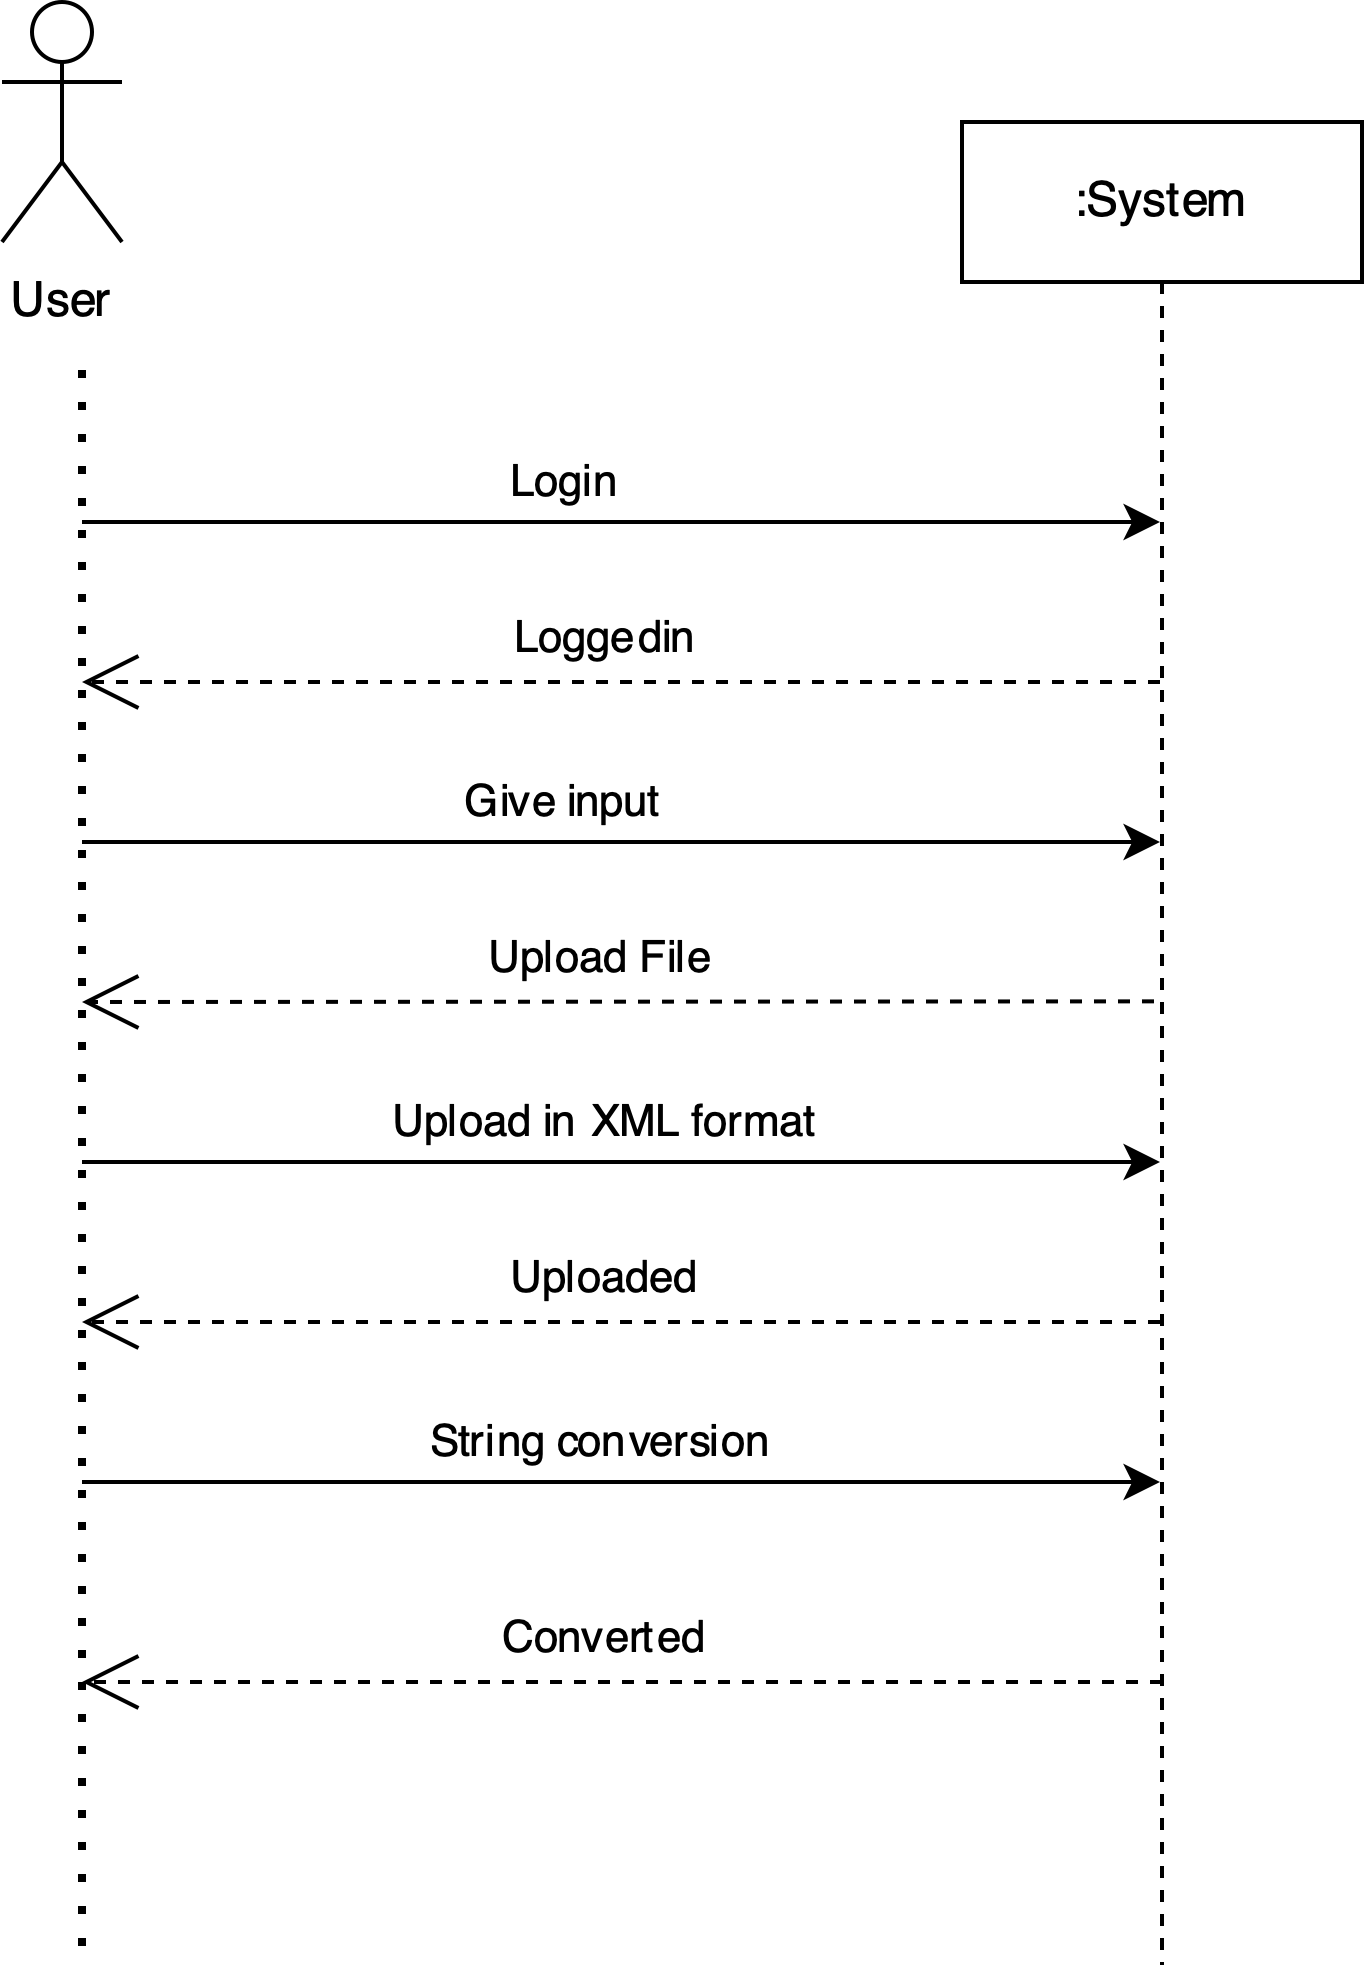
\includegraphics[scale=0.30]{Diagram/Login_SSD.png}
\caption{SSD-01 Login and input}
\end{figure}

\newpage
\subsection{Check Errors}
\begin{figure}[h]
 \centering
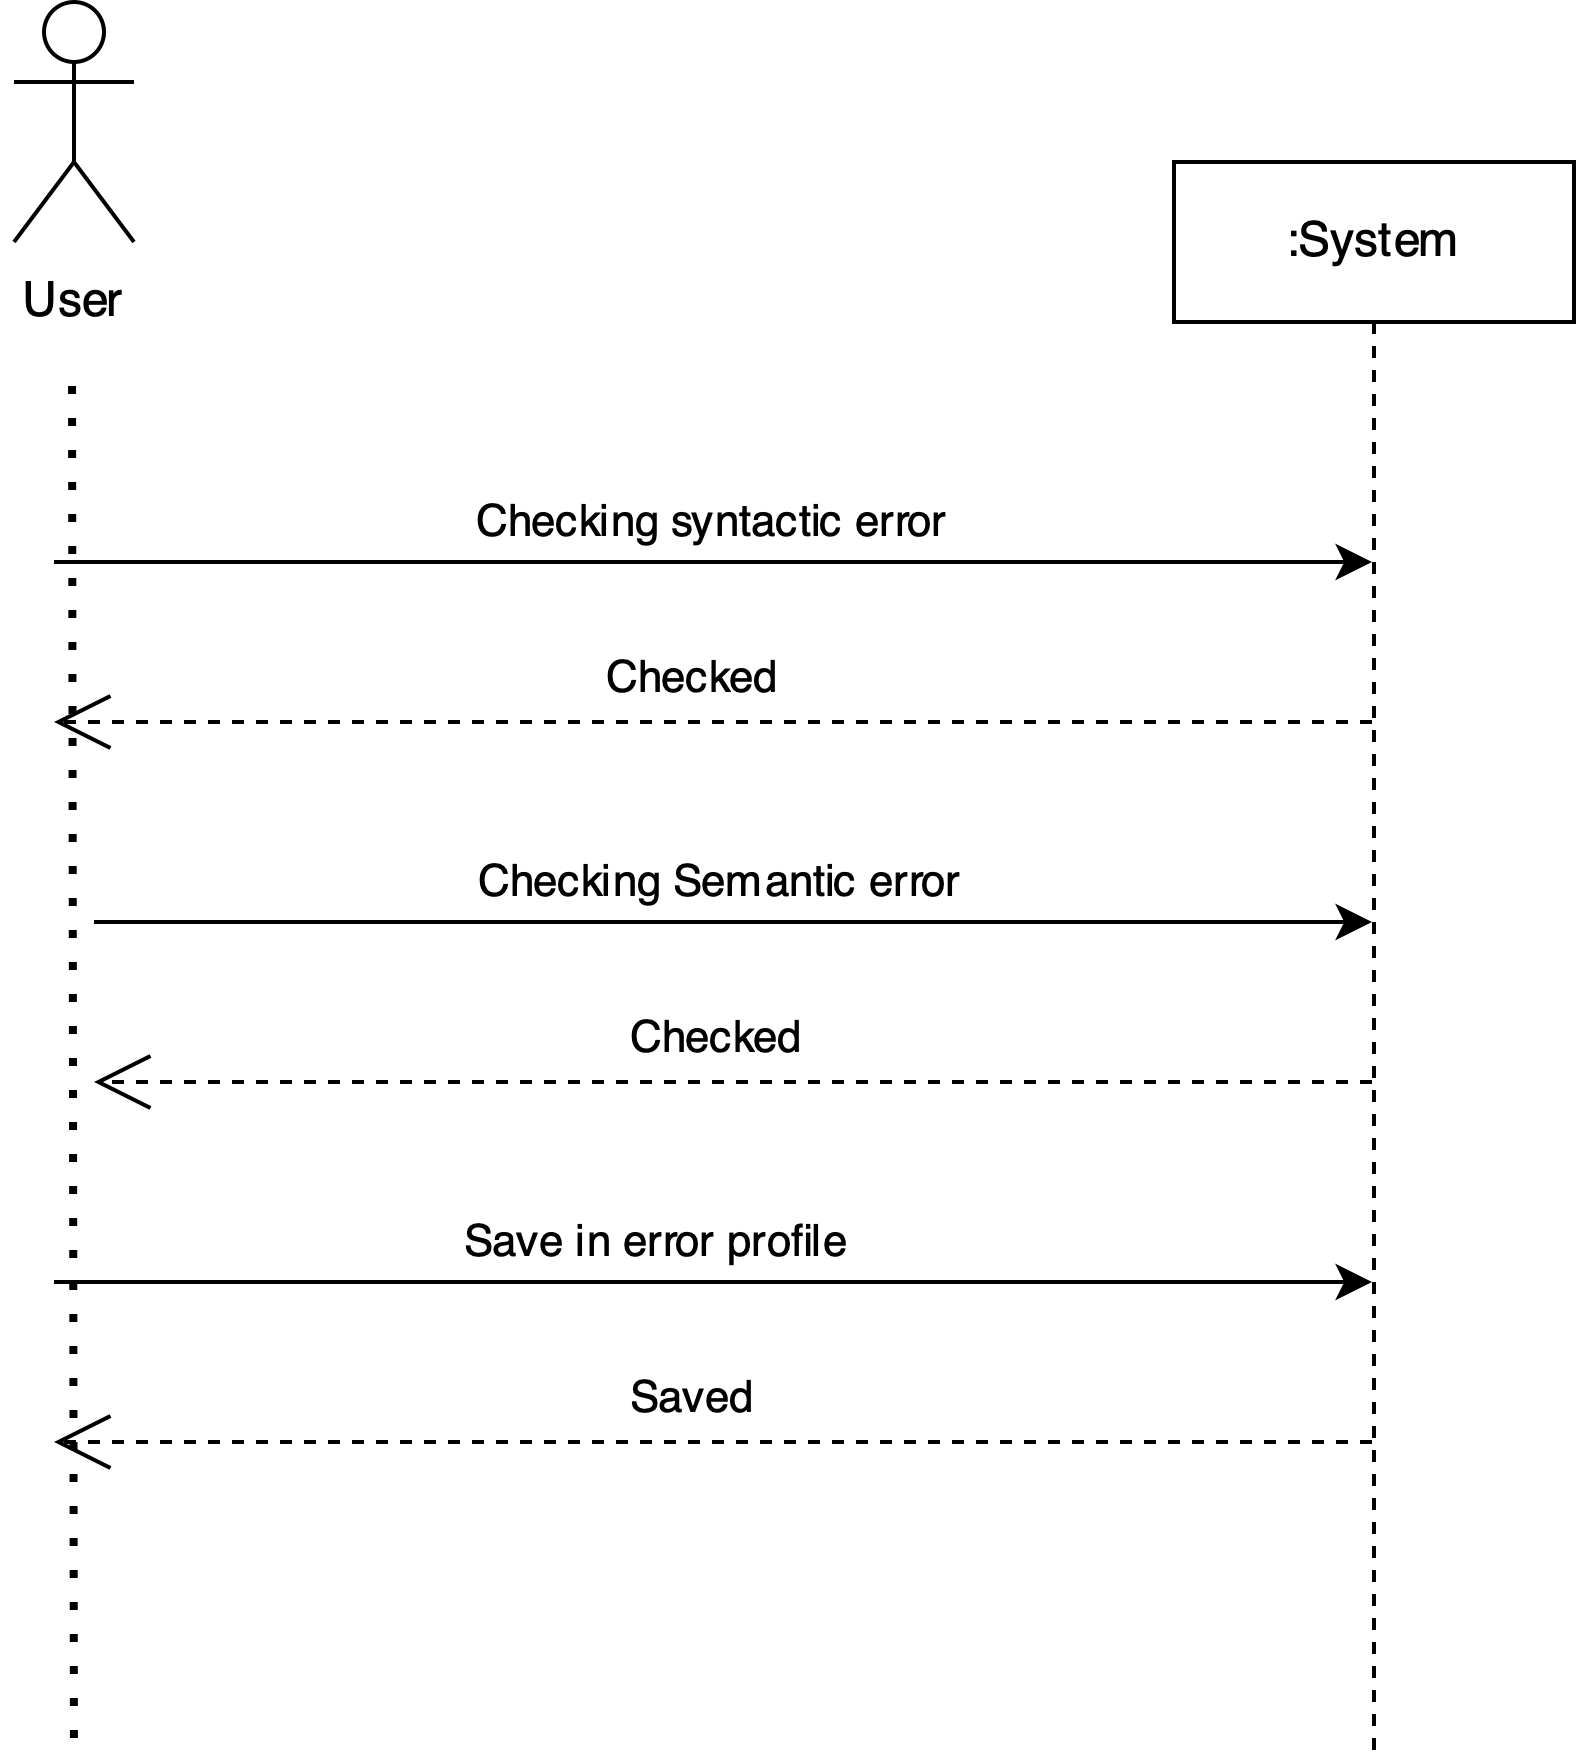
\includegraphics[scale=0.30]{Diagram/CheckingError_SSD.png}
\caption{SSD-02 Check Error}
\end{figure}
\newpage
\subsection{Admin}
\begin{figure}[h]
 \centering
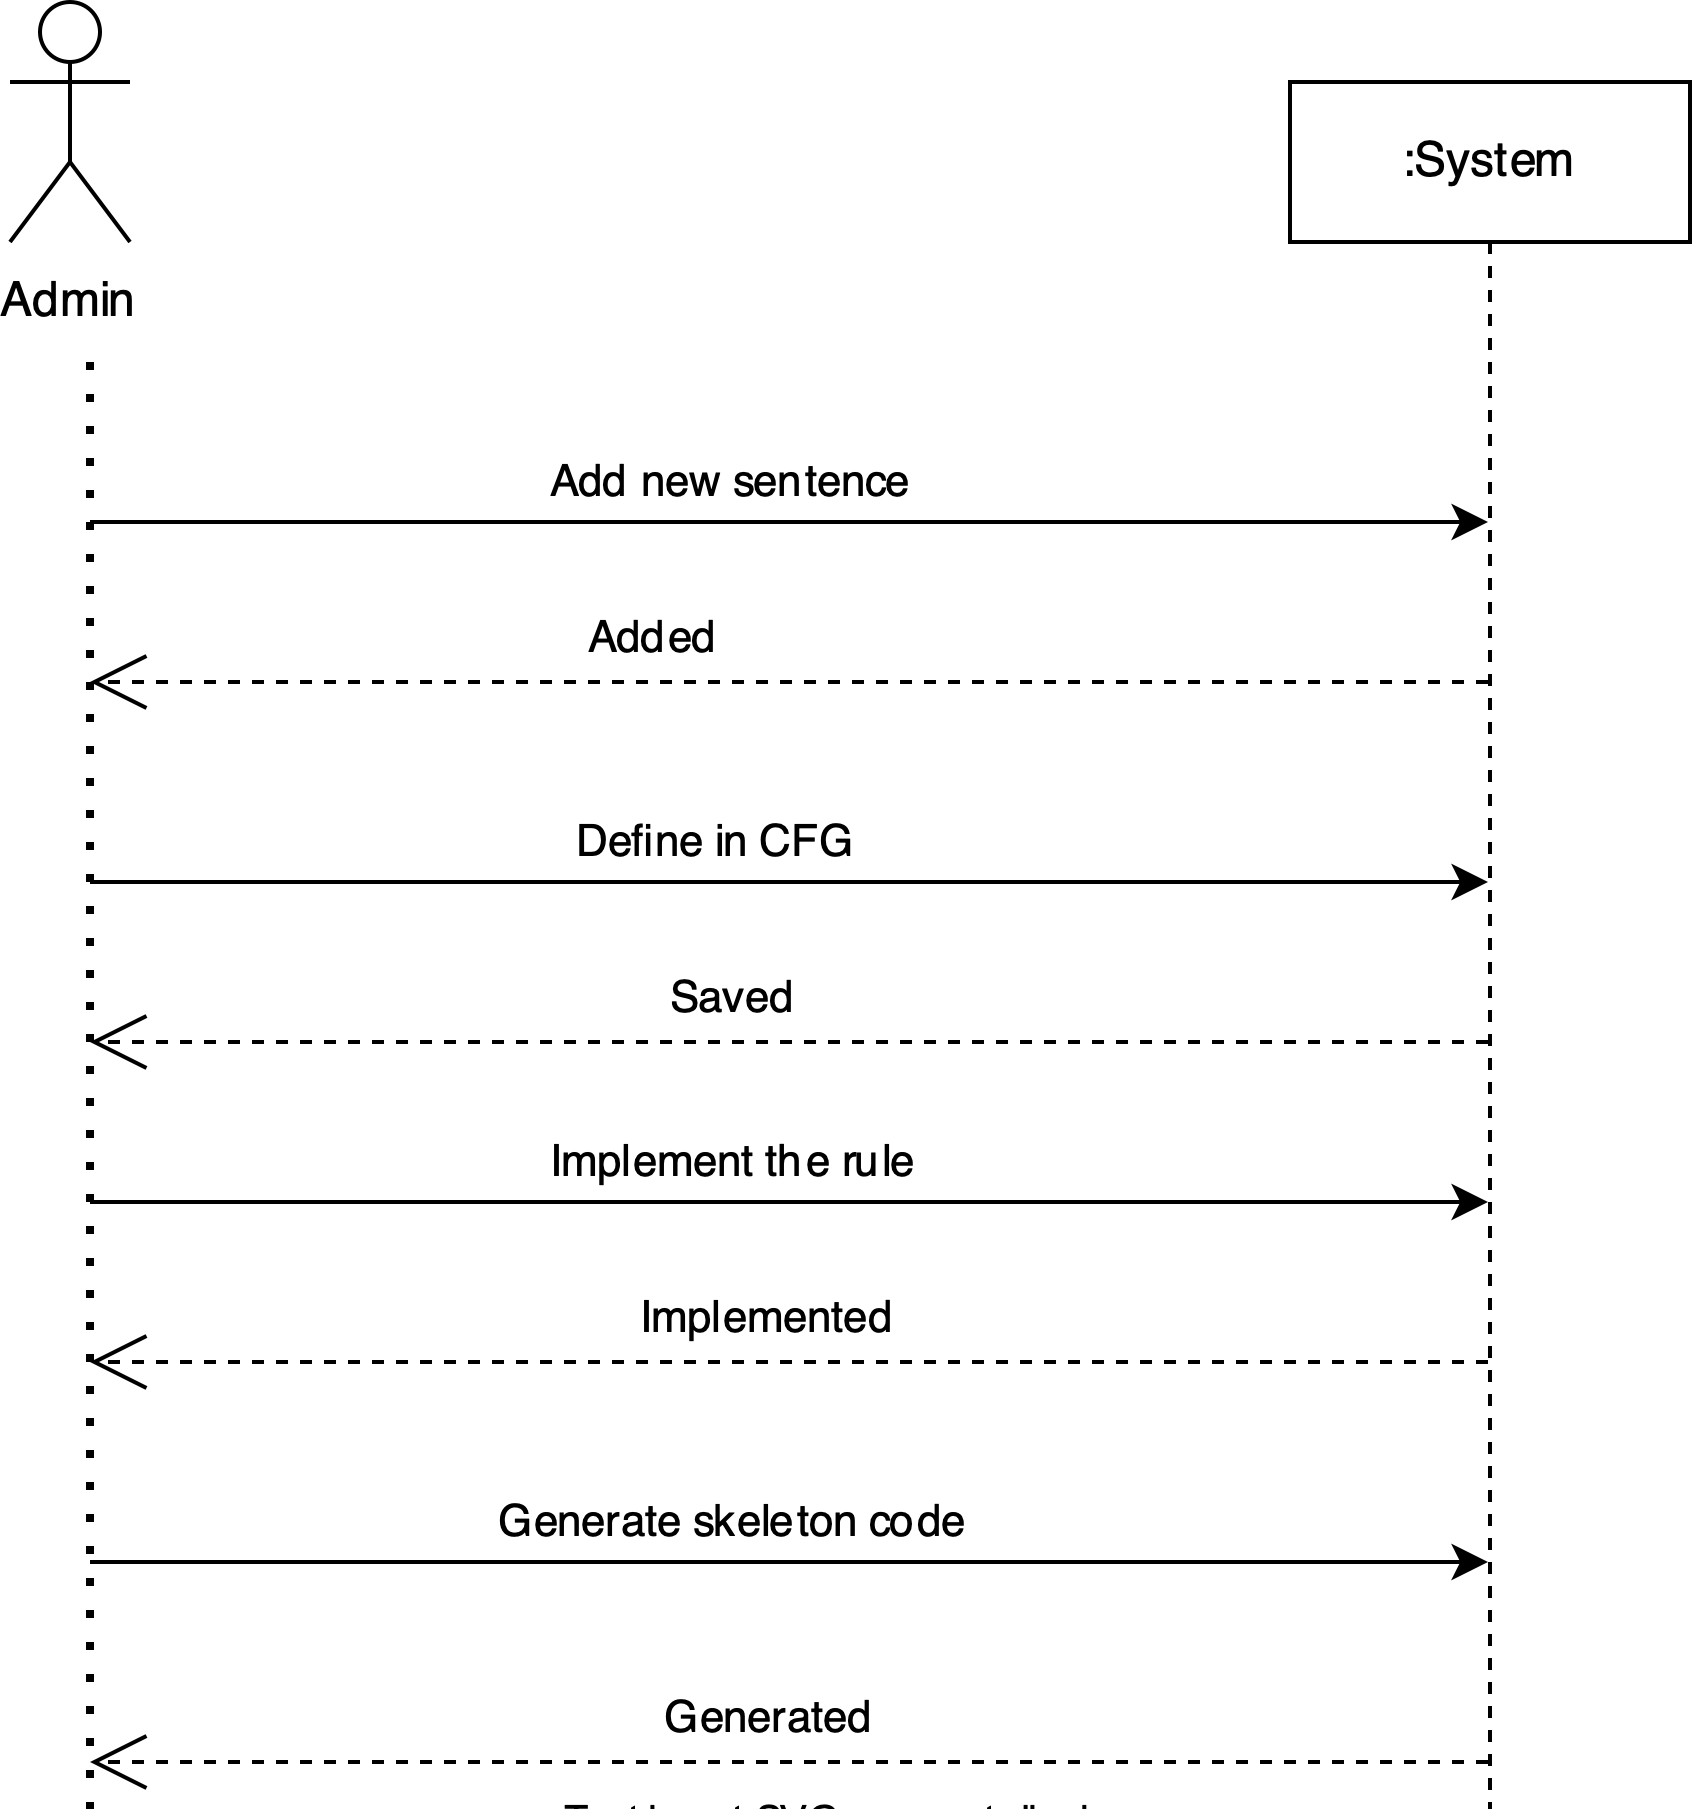
\includegraphics[scale=0.30]{Diagram/Admin_SSD.png}
\caption{SSD-03 Admin}
\end{figure}
% -------------ACTIVITY DIAGRAM---------------------------------------------------------------- 
\newpage
\section{Activity Diagram}
\subsection{Admin}
\begin{figure}[hb]
 \centering
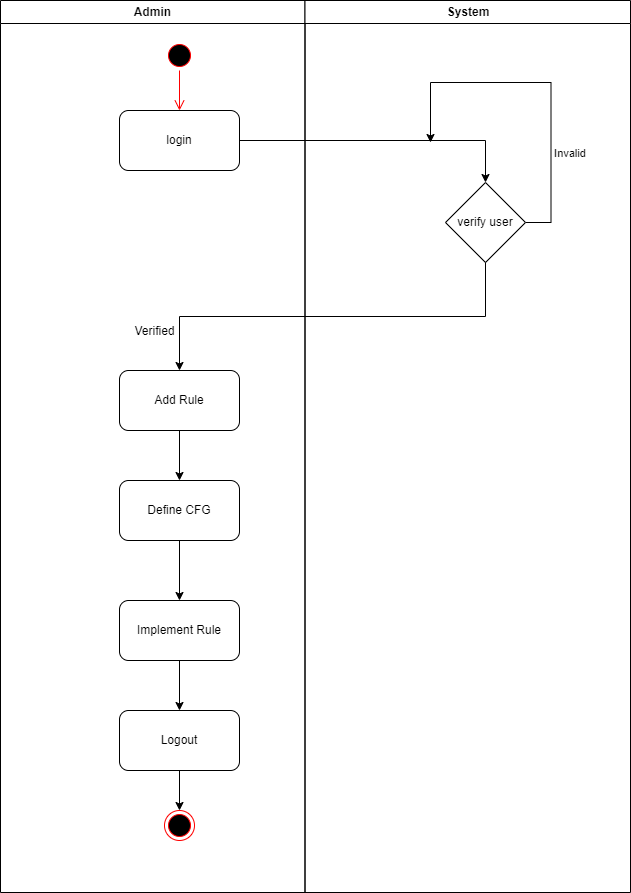
\includegraphics[scale=0.57]{Diagram/Admin_Activity_Diagram.png}
\caption{AD-01 Admin}
\end{figure}

\newpage
\subsection{User Input}
\begin{figure}[hb]
 \centering
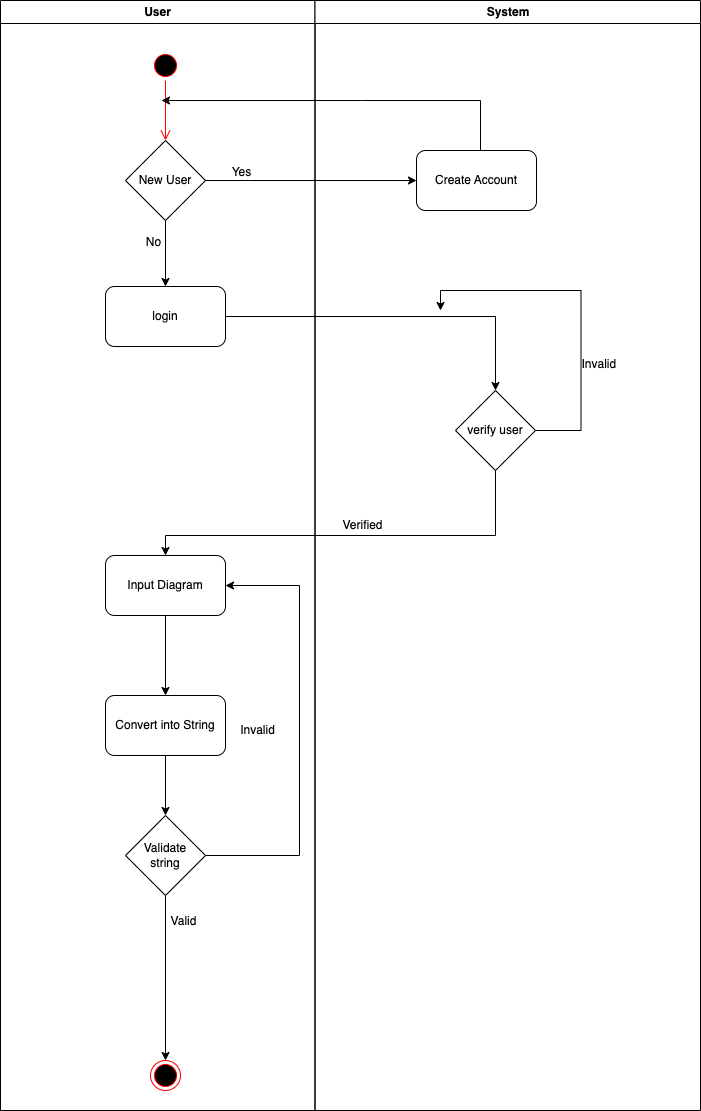
\includegraphics[scale=0.46]{Diagram/Input_Activity_Diagram.png}
\caption{AD-02 User Input}
\end{figure}
\newpage
\subsection{Check Error}
\begin{figure}[hb]
 \centering
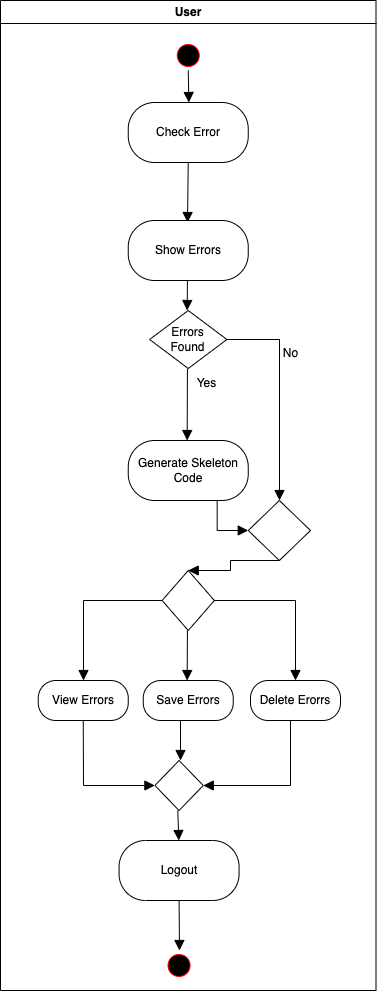
\includegraphics[scale=0.50]{Diagram/Checking_Error.drawio.png}
\caption{AD-03 Check Error}
\end{figure}

% -------------DOMAIN MODEL------------------------------------------------------------------
\newpage
\section{Domain Model}
\begin{figure}[h]
  \centering
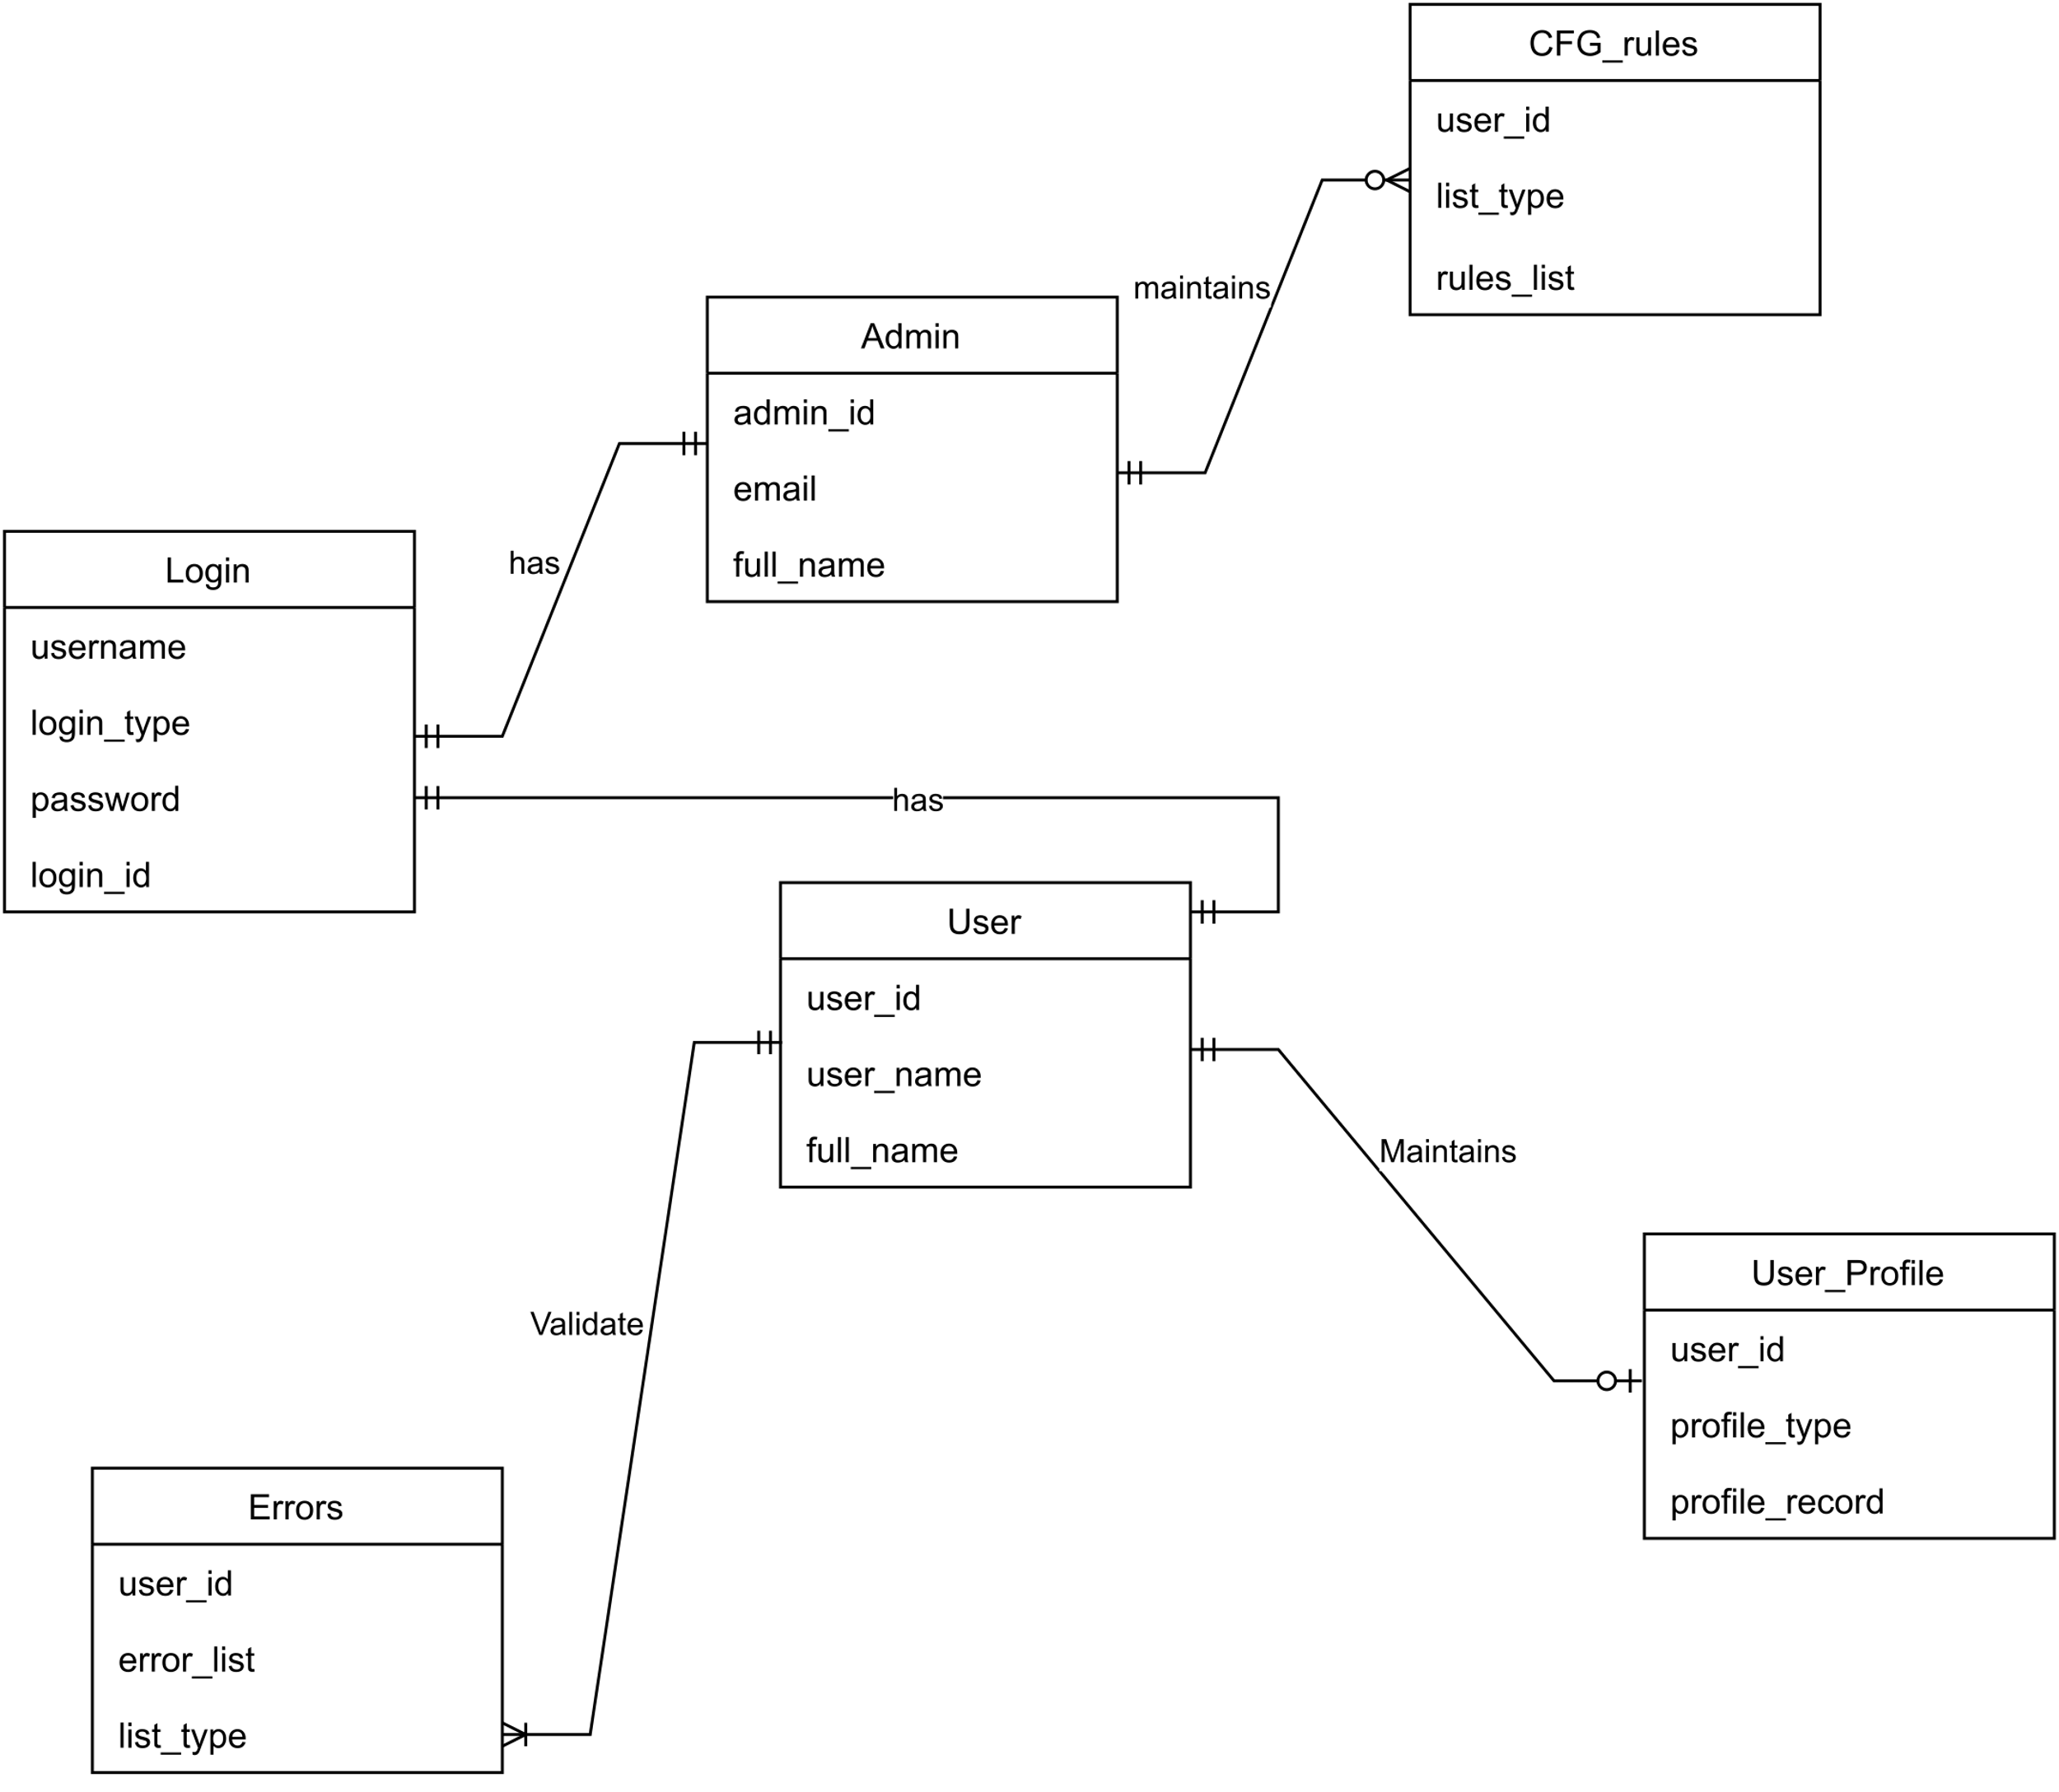
\includegraphics[width=\textwidth]{Diagram/Domain_Model.png}
\caption{Domain Model}
 \end{figure}
 % -------------CLASS DIAGRAM------------------------------------------------------------------   
\newpage
\section{Class Diagram}
\begin{figure}[h]
 \centering
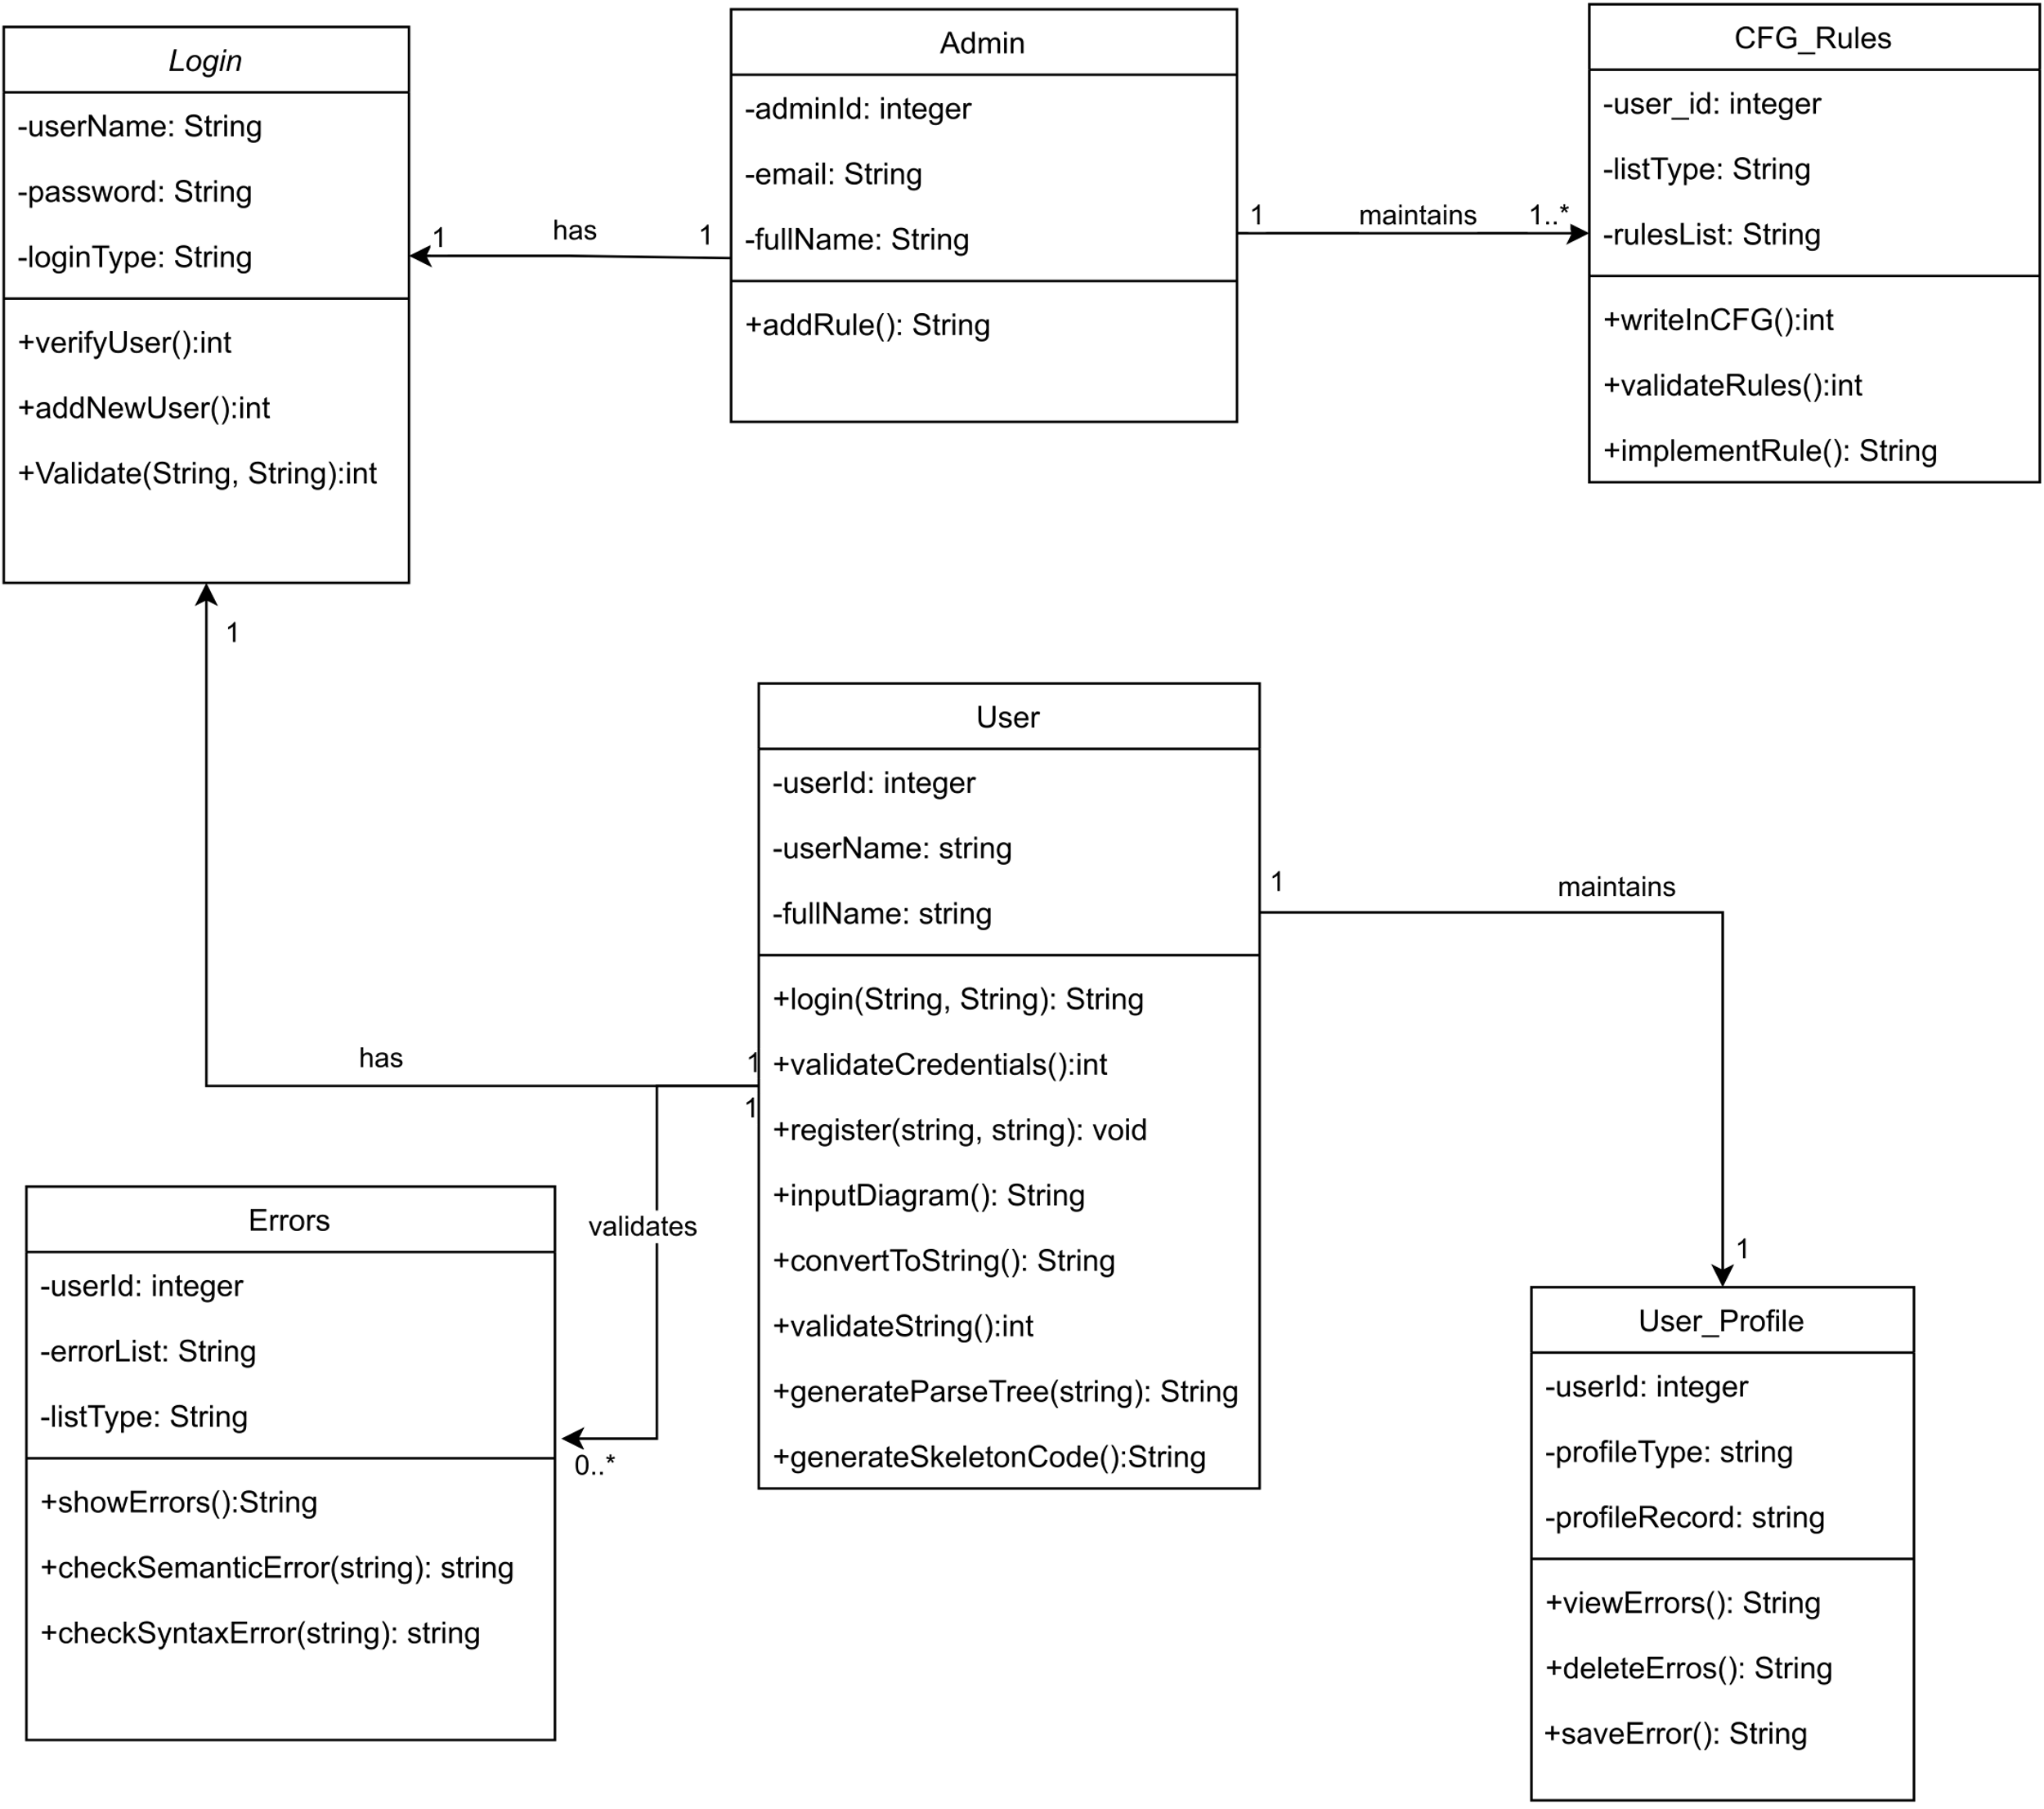
\includegraphics[scale=0.85]{Diagram/Class_Diagram.png}
\caption{Class Diagram}
\end{figure}

%-------------SEQUENCE DIAGRAM------------------------------------------------------------------
\newpage
\section{Sequence Diagram}
\subsection{Person Sign-up}
\begin{figure}[h]
 \centering
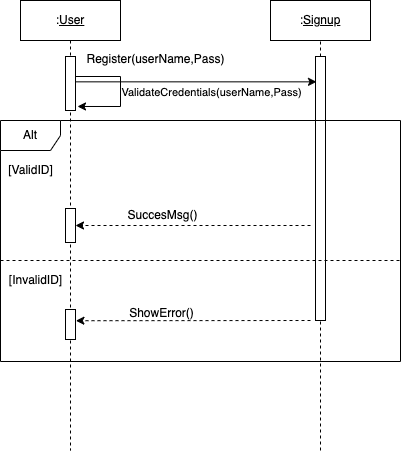
\includegraphics[scale=0.80]{Diagram/Signup Sequence Diagram.png}
\caption{SD-01 Person Sign-up}
\end{figure}

\newpage
\subsection{Person Login}
\begin{figure}[h]
 \centering
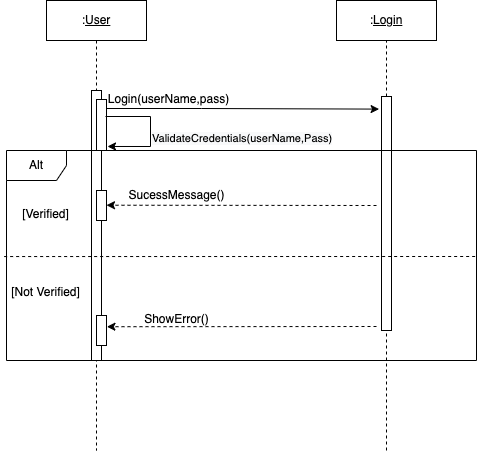
\includegraphics[scale=0.80]{Diagram/Login Sequence Diagram_NEW.png}
\caption{SD-02 Person Login}
\end{figure}

\newpage
\subsection{Take XML Format}
\begin{figure}[h]
 \centering
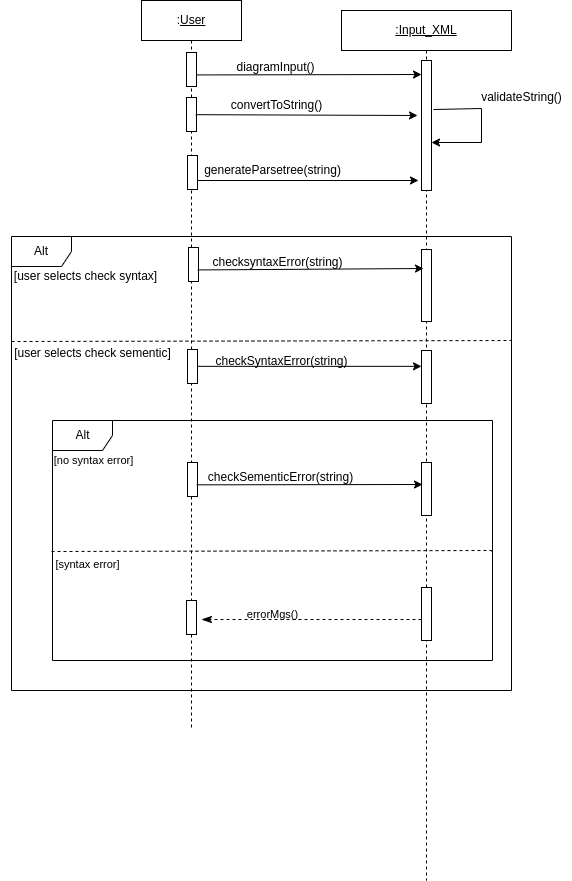
\includegraphics[scale=0.55]{Diagram/Take XML errors-checking errors-checking errors.drawio.png}
\caption{SD-03 Take XML Format}
\end{figure}
\newpage
\subsection{Release New Sentence}
\begin{figure}[h]
 \centering
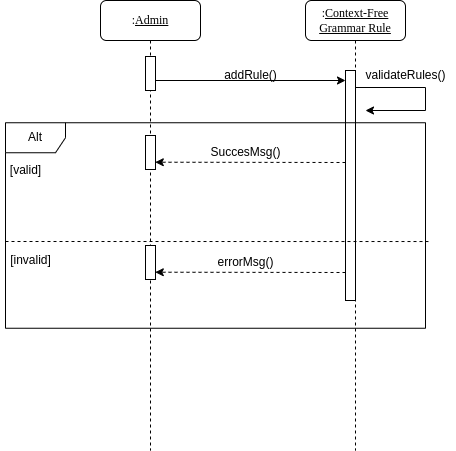
\includegraphics[scale=0.80]{Diagram/New_relesRule.png}
\caption{SD-04 Release New Sentence}
\end{figure}




% -------------ER DIAGRAM------------------------------------------------------------------
\newpage
\section{Entity Relation Diagram}

\begin{figure}[hb]
 \centering
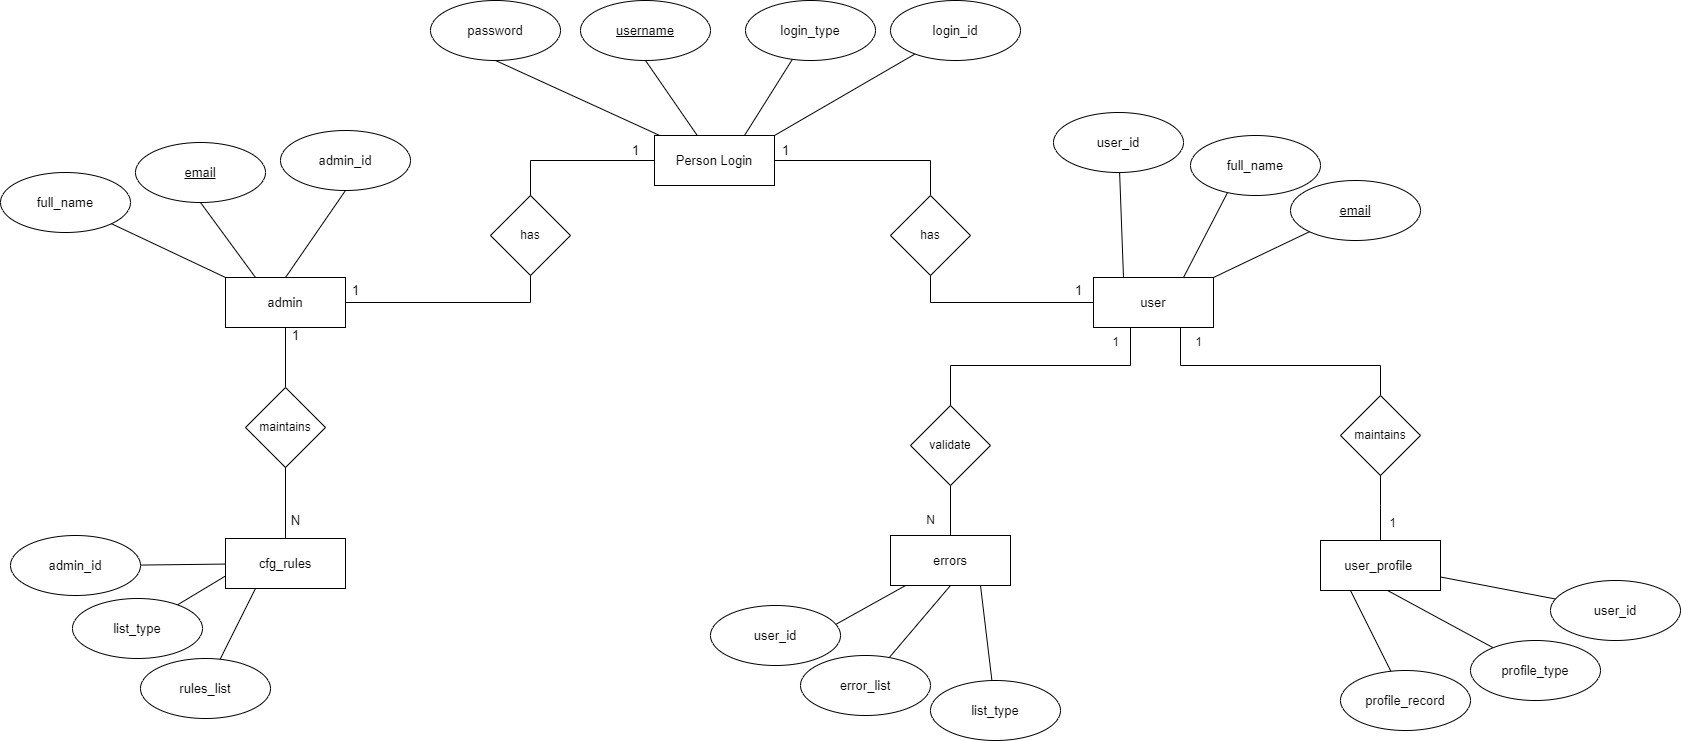
\includegraphics[scale=0.33]{Diagram/ER_Diagram.png}
\caption{Entity Relation Diagram}
\end{figure}



% -------------Database Logical Model------------------------------------------------------------------
% \newpage
% \section{Database Logical Model}
% \begin{figure}[h]
%  \centering
% 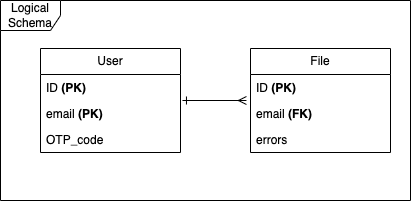
\includegraphics[scale=0.90]{Diagram/Logical_Schema.png}
% \caption{Logical Schema}
% \end{figure}
% -------------Database Physical Model------------------------------------------------------------------
% \newpage
% \section{Database Physical Model}


% -------------ARCHITECTURE  DIAGRAM------------------------------------------------------------------
\newpage
\section{Architecture Diagram}
\begin{figure}[h]
 \centering
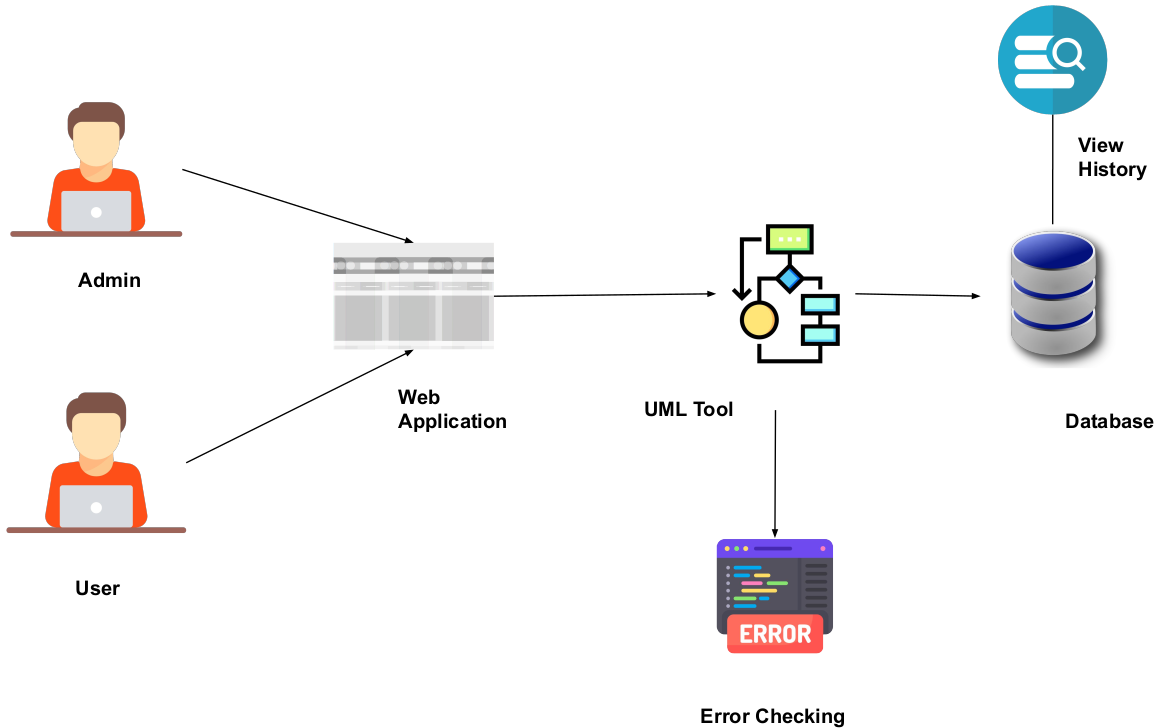
\includegraphics[scale=0.44]{Diagram/Architectyre Diagram.png}
\caption{Architecture Diagram}
\end{figure}
% -------------Test Cases------------------------------------------------------------------
\newpage
\section{Test Cases}
\subsection{Login}
    \begin{table}[h]
\caption{TC-01 Login}
    \centering
    \begin{tabular}{|p{9em}|p{9em}|p{4em}|p{4em}|p{4em}|}
    \hline
   \textbf{Test case ID}&\textbf{Input Values}&\textbf{Expected Output}
&\textbf{Actual Output}
&\textbf{Pass/Fail Status} \\%end of row
       \hline
     Valid Username and password &email=xyz.@gmail.com,
     \newline password=abc@&Login Successful&Login Successful&Passed \\%end of row
       \hline
      Invalid Username &email=123@gmail.com&nvalide Email format&Invalid Email format&Passed \\%end of row
       \hline
      Invalid password  &password=>/dkaxasd&Password does not match.Try again!&The password does not match.Try again!&Passed \\%end of row
       \hline
       Empty username and password field &email= ,password=&Fill the fields&Fill the fields&Passed \\%end of row
       \hline
       Password with incorrect case &email=123@gmail.com, password=./dkasda&Invalid Credentials&Invalid Credentials&Passed \\%end of row
       \hline
    \end{tabular} 
    \end{table}


\newpage
    \subsection{Database Connection}
    \begin{table}[h]
\caption{TC-02 Database Connection}
    \centering
    \begin{tabular}{|p{9em}|p{9em}|p{4em}|p{4em}|p{4em}|}
    \hline
   \textbf{Test case ID}&\textbf{Input Values}&\textbf{Expected Output}
&\textbf{Actual Output}
&\textbf{Pass/Fail Status} \\%end of row
       \hline
   Database connection &Var connection=\newline mysql.createConnection\newline(vars)&SQL CONNECT SUCCESSFUL&SQL CONNECT SUCCESSFUL&Passed\\
    \hline
     Database Validation &Var interval =setInterval(function(){
connection.ping()
}
&Ping successful&Ping successful&Passed\\
    \hline
     Database Security checks &Exceptional Handling&Securely transferring the data&No output&Does not exist\\
    \hline
   \end{tabular} 
    \end{table}



    
    \subsection{Node js}
    \begin{table}[h]
\caption{TC-03 Node js}
    \centering
    \begin{tabular}{|p{9em}|p{9em}|p{4em}|p{4em}|p{4em}|}
    \hline
   \textbf{Test case ID}&\textbf{Input Values}&\textbf{Expected Output}
&\textbf{Actual Output}
&\textbf{Pass/Fail Status} \\%end of row
       \hline
   Functionality  &&All working fine&Working&Passed\\
    \hline
    Error handling&If(err)=console.log() else console.log()&Errors are handled execute&Errors are handled&Passed\\
    \hline
     Asynchronous&loginUser=async()&Await,promises execute&Executing in normal flow&Passed\\
    \hline
    \end{tabular} 
    \end{table}


\newpage
\subsection{Express Route}
\begin{table}[h]
\caption{TC-04 Node Express Route}
\centering
\begin{tabular}{|p{9em}|p{9em}|p{4em}|p{4em}|p{4em}|}
\hline
\textbf{Test case ID}&\textbf{Input Values}&\textbf{Expected Output}
&\textbf{Actual Output}
&\textbf{Pass/Fail Status} \\%end of row
\hline
Successful Request&router.post(“/login”)&Requesting works&Routing &Passed\\
\hline
Invalid Request&router\newline.post(“/directory”)&Some Error occur&Some Error occur&Passed\\
\hline
Error Handling&if(err){console.log(err)}
&Handling errors&Some Error occur&Passed\\
\hline
Authentication&sql2=(\$(email),\$(pass)&Some error occur in checking email&Some error occur in checking email&Passed\\
\hline
\end{tabular} 
\end{table}

     \subsection{XML Parsing}
    \begin{table}[h]
\caption{TC-05 XML Parsing}
    \centering
    \begin{tabular}{|p{9em}|p{9em}|p{4em}|p{4em}|p{4em}|}
    \hline
   \textbf{Test case ID}&\textbf{Input Values}&\textbf{Expected Output}
&\textbf{Actual Output}
&\textbf{Pass/Fail Status} \\%end of row
       \hline
   Valid XML &ReadFile(xml)&Handle file read error&File is valide&Passed\\
    \hline
     inflate XML &parser.pareseString(data)&Handling parsing error if any&retuning&Passed\\
    \hline
    XML Child and Parent &if(mxcellarray[i]=1)&It means its a class&It means its a class&Passed\\
    \hline
    XML schema validation &Into Class and attribute and methods&Differnetiate the classes&Differnetiate the class&Passed\\
    \hline
    \end{tabular} 
    \end{table}
    \newpage
    \section{References}
    \begin{itemize}
        \item \url{https://www.uml-diagrams.org/uml-25-diagrams.html}
        \item \url{https://nulab.com/learn/software-development/intro-uml-diagram-types-templates/}
        \item \url{http://www.cs.sjsu.edu/~pearce/modules/lectures/uml2/index.htm}
        \item \url{https://link.springer.com/chapter/10.1007/978-3-642-11659-9_22}
    \end{itemize}








    
    
\end{document}